\documentclass[twoside]{book}

% Packages required by doxygen
\usepackage{calc}
\usepackage{doxygen}
\usepackage{graphicx}
\usepackage[utf8]{inputenc}
\usepackage{makeidx}
\usepackage{multicol}
\usepackage{multirow}
\usepackage{textcomp}
\usepackage[table]{xcolor}

% Font selection
\usepackage[T1]{fontenc}
\usepackage{mathptmx}
\usepackage[scaled=.90]{helvet}
\usepackage{courier}
\usepackage{amssymb}
\usepackage{sectsty}
\renewcommand{\familydefault}{\sfdefault}
\allsectionsfont{%
  \fontseries{bc}\selectfont%
  \color{darkgray}%
}
\renewcommand{\DoxyLabelFont}{%
  \fontseries{bc}\selectfont%
  \color{darkgray}%
}

% Page & text layout
\usepackage{geometry}
\geometry{%
  a4paper,%
  top=2.5cm,%
  bottom=2.5cm,%
  left=2.5cm,%
  right=2.5cm%
}
\tolerance=750
\hfuzz=15pt
\hbadness=750
\setlength{\emergencystretch}{15pt}
\setlength{\parindent}{0cm}
\setlength{\parskip}{0.2cm}
\makeatletter
\renewcommand{\paragraph}{%
  \@startsection{paragraph}{4}{0ex}{-1.0ex}{1.0ex}{%
    \normalfont\normalsize\bfseries\SS@parafont%
  }%
}
\renewcommand{\subparagraph}{%
  \@startsection{subparagraph}{5}{0ex}{-1.0ex}{1.0ex}{%
    \normalfont\normalsize\bfseries\SS@subparafont%
  }%
}
\makeatother

% Headers & footers
\usepackage{fancyhdr}
\pagestyle{fancyplain}
\fancyhead[LE]{\fancyplain{}{\bfseries\thepage}}
\fancyhead[CE]{\fancyplain{}{}}
\fancyhead[RE]{\fancyplain{}{\bfseries\leftmark}}
\fancyhead[LO]{\fancyplain{}{\bfseries\rightmark}}
\fancyhead[CO]{\fancyplain{}{}}
\fancyhead[RO]{\fancyplain{}{\bfseries\thepage}}
\fancyfoot[LE]{\fancyplain{}{}}
\fancyfoot[CE]{\fancyplain{}{}}
\fancyfoot[RE]{\fancyplain{}{\bfseries\scriptsize Generated on Wed Nov 27 2013 19:35:18 for Stickman Project by Doxygen }}
\fancyfoot[LO]{\fancyplain{}{\bfseries\scriptsize Generated on Wed Nov 27 2013 19:35:18 for Stickman Project by Doxygen }}
\fancyfoot[CO]{\fancyplain{}{}}
\fancyfoot[RO]{\fancyplain{}{}}
\renewcommand{\footrulewidth}{0.4pt}
\renewcommand{\chaptermark}[1]{%
  \markboth{#1}{}%
}
\renewcommand{\sectionmark}[1]{%
  \markright{\thesection\ #1}%
}

% Indices & bibliography
\usepackage{natbib}
\usepackage[titles]{tocloft}
\setcounter{tocdepth}{3}
\setcounter{secnumdepth}{5}
\makeindex

% Hyperlinks (required, but should be loaded last)
\usepackage{ifpdf}
\ifpdf
  \usepackage[pdftex,pagebackref=true]{hyperref}
\else
  \usepackage[ps2pdf,pagebackref=true]{hyperref}
\fi
\hypersetup{%
  colorlinks=true,%
  linkcolor=blue,%
  citecolor=blue,%
  unicode%
}

% Custom commands
\newcommand{\clearemptydoublepage}{%
  \newpage{\pagestyle{empty}\cleardoublepage}%
}


%===== C O N T E N T S =====

\begin{document}

% Titlepage & ToC
\hypersetup{pageanchor=false}
\pagenumbering{roman}
\begin{titlepage}
\vspace*{7cm}
\begin{center}%
{\Large Stickman Project \\[1ex]\large 1.\-0 }\\
\vspace*{1cm}
{\large Generated by Doxygen 1.8.4}\\
\vspace*{0.5cm}
{\small Wed Nov 27 2013 19:35:18}\\
\end{center}
\end{titlepage}
\clearemptydoublepage
\tableofcontents
\clearemptydoublepage
\pagenumbering{arabic}
\hypersetup{pageanchor=true}

%--- Begin generated contents ---
\chapter{Hierarchical Index}
\section{Class Hierarchy}
This inheritance list is sorted roughly, but not completely, alphabetically\-:\begin{DoxyCompactList}
\item \contentsline{section}{A\-Factory}{\pageref{class_a_factory}}{}
\begin{DoxyCompactList}
\item \contentsline{section}{Concrete\-Factory}{\pageref{class_concrete_factory}}{}
\end{DoxyCompactList}
\item \contentsline{section}{Game\-Manager}{\pageref{class_game_manager}}{}
\item \contentsline{section}{I\-Block}{\pageref{class_i_block}}{}
\begin{DoxyCompactList}
\item \contentsline{section}{Block\-Ground1}{\pageref{class_block_ground1}}{}
\item \contentsline{section}{Block\-Ground2}{\pageref{class_block_ground2}}{}
\item \contentsline{section}{Block\-Ground3}{\pageref{class_block_ground3}}{}
\end{DoxyCompactList}
\item \contentsline{section}{I\-Level}{\pageref{class_i_level}}{}
\begin{DoxyCompactList}
\item \contentsline{section}{Level\-One}{\pageref{class_level_one}}{}
\item \contentsline{section}{Level\-Two}{\pageref{class_level_two}}{}
\end{DoxyCompactList}
\item \contentsline{section}{Menu}{\pageref{class_menu}}{}
\item \contentsline{section}{Player}{\pageref{class_player}}{}
\begin{DoxyCompactList}
\item \contentsline{section}{A\-Upgrade}{\pageref{class_a_upgrade}}{}
\begin{DoxyCompactList}
\item \contentsline{section}{Cape}{\pageref{class_cape}}{}
\item \contentsline{section}{Shoes}{\pageref{class_shoes}}{}
\end{DoxyCompactList}
\end{DoxyCompactList}
\end{DoxyCompactList}

\chapter{Class Index}
\section{Class List}
Here are the classes, structs, unions and interfaces with brief descriptions\-:\begin{DoxyCompactList}
\item\contentsline{section}{\hyperlink{class_a_factory}{A\-Factory} \\*Provide a factory to create blocks }{\pageref{class_a_factory}}{}
\item\contentsline{section}{\hyperlink{class_a_upgrade}{A\-Upgrade} \\*Abstract class for the upgrades }{\pageref{class_a_upgrade}}{}
\item\contentsline{section}{\hyperlink{class_block_ground1}{Block\-Ground1} \\*A concrete block that implements \hyperlink{class_i_block}{I\-Block} }{\pageref{class_block_ground1}}{}
\item\contentsline{section}{\hyperlink{class_block_ground2}{Block\-Ground2} \\*Another concrete block that implements \hyperlink{class_i_block}{I\-Block} }{\pageref{class_block_ground2}}{}
\item\contentsline{section}{\hyperlink{class_block_ground3}{Block\-Ground3} \\*Another concrete block that implements \hyperlink{class_i_block}{I\-Block} }{\pageref{class_block_ground3}}{}
\item\contentsline{section}{\hyperlink{class_cape}{Cape} \\*\hyperlink{class_cape}{Cape} upgrade }{\pageref{class_cape}}{}
\item\contentsline{section}{\hyperlink{class_concrete_factory}{Concrete\-Factory} \\*A concrete factory to create blocks }{\pageref{class_concrete_factory}}{}
\item\contentsline{section}{\hyperlink{class_game_manager}{Game\-Manager} \\*Provide an instance to manage the game }{\pageref{class_game_manager}}{}
\item\contentsline{section}{\hyperlink{class_i_block}{I\-Block} \\*Interface that will be implemented by all the different kinds of blocks }{\pageref{class_i_block}}{}
\item\contentsline{section}{\hyperlink{class_i_level}{I\-Level} \\*Interface that will be implemented by the levels }{\pageref{class_i_level}}{}
\item\contentsline{section}{\hyperlink{class_level_one}{Level\-One} \\*Implements the first level of the game }{\pageref{class_level_one}}{}
\item\contentsline{section}{\hyperlink{class_level_two}{Level\-Two} \\*Implements the second level of the game }{\pageref{class_level_two}}{}
\item\contentsline{section}{\hyperlink{class_menu}{Menu} \\*Game menu }{\pageref{class_menu}}{}
\item\contentsline{section}{\hyperlink{class_player}{Player} \\*\hyperlink{class_player}{Player} class }{\pageref{class_player}}{}
\item\contentsline{section}{\hyperlink{class_shoes}{Shoes} \\*\hyperlink{class_shoes}{Shoes} class }{\pageref{class_shoes}}{}
\end{DoxyCompactList}

\chapter{File Index}
\section{File List}
Here is a list of all documented files with brief descriptions\-:\begin{DoxyCompactList}
\item\contentsline{section}{include/\-Decorator/\hyperlink{_a_upgrade_8h}{A\-Upgrade.\-h} }{\pageref{_a_upgrade_8h}}{}
\item\contentsline{section}{include/\-Decorator/\hyperlink{_cape_8h}{Cape.\-h} }{\pageref{_cape_8h}}{}
\item\contentsline{section}{include/\-Decorator/\hyperlink{_player_8h}{Player.\-h} }{\pageref{_player_8h}}{}
\item\contentsline{section}{include/\-Decorator/\hyperlink{_shoes_8h}{Shoes.\-h} }{\pageref{_shoes_8h}}{}
\item\contentsline{section}{include/\-Factory/\hyperlink{_a_factory_8h}{A\-Factory.\-h} }{\pageref{_a_factory_8h}}{}
\item\contentsline{section}{include/\-Factory/\hyperlink{_block_ground1_8h}{Block\-Ground1.\-h} }{\pageref{_block_ground1_8h}}{}
\item\contentsline{section}{include/\-Factory/\hyperlink{_block_ground2_8h}{Block\-Ground2.\-h} }{\pageref{_block_ground2_8h}}{}
\item\contentsline{section}{include/\-Factory/\hyperlink{_block_ground3_8h}{Block\-Ground3.\-h} }{\pageref{_block_ground3_8h}}{}
\item\contentsline{section}{include/\-Factory/\hyperlink{_concrete_factory_8h}{Concrete\-Factory.\-h} }{\pageref{_concrete_factory_8h}}{}
\item\contentsline{section}{include/\-Factory/\hyperlink{_i_block_8h}{I\-Block.\-h} }{\pageref{_i_block_8h}}{}
\item\contentsline{section}{include/\-Singleton/\hyperlink{_game_manager_8h}{Game\-Manager.\-h} }{\pageref{_game_manager_8h}}{}
\item\contentsline{section}{include/\-Singleton/\hyperlink{_menu_8h}{Menu.\-h} }{\pageref{_menu_8h}}{}
\item\contentsline{section}{include/\-Strategy/\hyperlink{_i_level_8h}{I\-Level.\-h} }{\pageref{_i_level_8h}}{}
\item\contentsline{section}{include/\-Strategy/\hyperlink{_level_one_8h}{Level\-One.\-h} }{\pageref{_level_one_8h}}{}
\item\contentsline{section}{include/\-Strategy/\hyperlink{_level_two_8h}{Level\-Two.\-h} }{\pageref{_level_two_8h}}{}
\end{DoxyCompactList}

\chapter{Class Documentation}
\hypertarget{class_a_factory}{\section{A\-Factory Class Reference}
\label{class_a_factory}\index{A\-Factory@{A\-Factory}}
}


Provide a factory to create blocks.  




Inheritance diagram for A\-Factory\-:\nopagebreak
\begin{figure}[H]
\begin{center}
\leavevmode
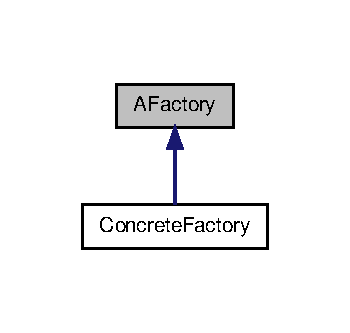
\includegraphics[width=168pt]{class_a_factory__inherit__graph}
\end{center}
\end{figure}
\subsection*{Public Member Functions}
\begin{DoxyCompactItemize}
\item 
\hypertarget{class_a_factory_a5c61aa93311f5ffe67ef07f24375e548}{virtual \hyperlink{class_a_factory_a5c61aa93311f5ffe67ef07f24375e548}{$\sim$\-A\-Factory} ()}\label{class_a_factory_a5c61aa93311f5ffe67ef07f24375e548}

\begin{DoxyCompactList}\small\item\em Default destructor. \end{DoxyCompactList}\item 
\hyperlink{class_i_block}{I\-Block} $\ast$ \hyperlink{class_a_factory_ac0e9f907f902b54796047020683b81e9}{create\-Block} (char c)
\begin{DoxyCompactList}\small\item\em Create a block using the \hyperlink{class_a_factory_adec2bf9f81dbf37ef727bcfb43403867}{build()} method. \end{DoxyCompactList}\item 
virtual \hyperlink{class_i_block}{I\-Block} $\ast$ \hyperlink{class_a_factory_adec2bf9f81dbf37ef727bcfb43403867}{build} (char s)=0
\begin{DoxyCompactList}\small\item\em Create a block according to the given character. \end{DoxyCompactList}\end{DoxyCompactItemize}
\subsection*{Protected Attributes}
\begin{DoxyCompactItemize}
\item 
\hypertarget{class_a_factory_a1d9a7f66cab1eaec378206e13fde820a}{\hyperlink{class_i_block}{I\-Block} $\ast$ \hyperlink{class_a_factory_a1d9a7f66cab1eaec378206e13fde820a}{m\-\_\-block}}\label{class_a_factory_a1d9a7f66cab1eaec378206e13fde820a}

\begin{DoxyCompactList}\small\item\em The block constructed. \end{DoxyCompactList}\end{DoxyCompactItemize}


\subsection{Detailed Description}
Provide a factory to create blocks. 

\begin{DoxyAuthor}{Author}
Adrien Bodineau and Alexandre Gomes 
\end{DoxyAuthor}
\begin{DoxyVersion}{Version}
1.\-0 
\end{DoxyVersion}


\subsection{Member Function Documentation}
\hypertarget{class_a_factory_adec2bf9f81dbf37ef727bcfb43403867}{\index{A\-Factory@{A\-Factory}!build@{build}}
\index{build@{build}!AFactory@{A\-Factory}}
\subsubsection[{build}]{\setlength{\rightskip}{0pt plus 5cm}{\bf I\-Block} $\ast$ A\-Factory\-::build (
\begin{DoxyParamCaption}
\item[{char}]{s}
\end{DoxyParamCaption}
)\hspace{0.3cm}{\ttfamily [pure virtual]}}}\label{class_a_factory_adec2bf9f81dbf37ef727bcfb43403867}


Create a block according to the given character. 


\begin{DoxyParams}{Parameters}
{\em s} & A char that indicate the block to construct \\
\hline
\end{DoxyParams}
\begin{DoxyReturn}{Returns}
The block constructed 
\end{DoxyReturn}


Implemented in \hyperlink{class_concrete_factory_a74d4adfe19116f2fbc31f1c3b745a297}{Concrete\-Factory}.

\hypertarget{class_a_factory_ac0e9f907f902b54796047020683b81e9}{\index{A\-Factory@{A\-Factory}!create\-Block@{create\-Block}}
\index{create\-Block@{create\-Block}!AFactory@{A\-Factory}}
\subsubsection[{create\-Block}]{\setlength{\rightskip}{0pt plus 5cm}{\bf I\-Block} $\ast$ A\-Factory\-::create\-Block (
\begin{DoxyParamCaption}
\item[{char}]{c}
\end{DoxyParamCaption}
)}}\label{class_a_factory_ac0e9f907f902b54796047020683b81e9}


Create a block using the \hyperlink{class_a_factory_adec2bf9f81dbf37ef727bcfb43403867}{build()} method. 


\begin{DoxyParams}{Parameters}
{\em c} & A char that indicate the block to construct \\
\hline
\end{DoxyParams}
\begin{DoxyReturn}{Returns}
The block constructed 
\end{DoxyReturn}

\hypertarget{class_a_upgrade}{\section{A\-Upgrade Class Reference}
\label{class_a_upgrade}\index{A\-Upgrade@{A\-Upgrade}}
}


Abstract class for the upgrades.  




Inheritance diagram for A\-Upgrade\-:\nopagebreak
\begin{figure}[H]
\begin{center}
\leavevmode
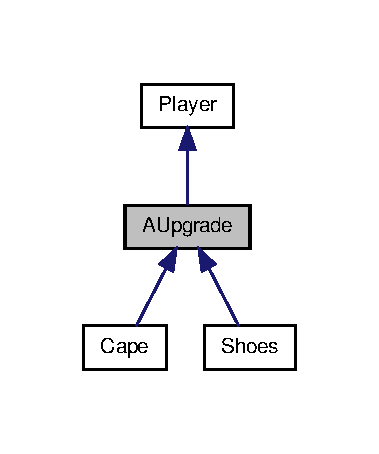
\includegraphics[width=182pt]{class_a_upgrade__inherit__graph}
\end{center}
\end{figure}
\subsection*{Public Member Functions}
\begin{DoxyCompactItemize}
\item 
\hypertarget{class_a_upgrade_a657c30a4f6115e0e4889791e16a55515}{\hyperlink{class_a_upgrade_a657c30a4f6115e0e4889791e16a55515}{A\-Upgrade} ()}\label{class_a_upgrade_a657c30a4f6115e0e4889791e16a55515}

\begin{DoxyCompactList}\small\item\em Default constructor. \end{DoxyCompactList}\item 
\hyperlink{class_a_upgrade_a1c08a05a63bbd9f90ea6ef96c662ed16}{A\-Upgrade} (\hyperlink{class_player}{Player} $\ast$character, int x, int y)
\begin{DoxyCompactList}\small\item\em Another constructor. \end{DoxyCompactList}\item 
\hypertarget{class_a_upgrade_abf739f8ff28186a086f751cf40a2fdbc}{virtual \hyperlink{class_a_upgrade_abf739f8ff28186a086f751cf40a2fdbc}{$\sim$\-A\-Upgrade} ()}\label{class_a_upgrade_abf739f8ff28186a086f751cf40a2fdbc}

\begin{DoxyCompactList}\small\item\em Default destructor. \end{DoxyCompactList}\end{DoxyCompactItemize}
\subsection*{Protected Attributes}
\begin{DoxyCompactItemize}
\item 
\hypertarget{class_a_upgrade_a66a92f5be2743d9317a7b3d82825dee6}{\hyperlink{class_player}{Player} $\ast$ \hyperlink{class_a_upgrade_a66a92f5be2743d9317a7b3d82825dee6}{m\-\_\-character}}\label{class_a_upgrade_a66a92f5be2743d9317a7b3d82825dee6}

\begin{DoxyCompactList}\small\item\em Decorated character. \end{DoxyCompactList}\end{DoxyCompactItemize}


\subsection{Detailed Description}
Abstract class for the upgrades. 

\begin{DoxyAuthor}{Author}
Adrien Bodineau and Alexandre Gomes 
\end{DoxyAuthor}
\begin{DoxyVersion}{Version}
1.\-0 
\end{DoxyVersion}


\subsection{Constructor \& Destructor Documentation}
\hypertarget{class_a_upgrade_a1c08a05a63bbd9f90ea6ef96c662ed16}{\index{A\-Upgrade@{A\-Upgrade}!A\-Upgrade@{A\-Upgrade}}
\index{A\-Upgrade@{A\-Upgrade}!AUpgrade@{A\-Upgrade}}
\subsubsection[{A\-Upgrade}]{\setlength{\rightskip}{0pt plus 5cm}A\-Upgrade\-::\-A\-Upgrade (
\begin{DoxyParamCaption}
\item[{{\bf Player} $\ast$}]{character, }
\item[{int}]{x, }
\item[{int}]{y}
\end{DoxyParamCaption}
)}}\label{class_a_upgrade_a1c08a05a63bbd9f90ea6ef96c662ed16}


Another constructor. 


\begin{DoxyParams}{Parameters}
{\em character} & Decorated character \\
\hline
{\em x} & Position x \\
\hline
{\em y} & Position y \\
\hline
\end{DoxyParams}

\hypertarget{class_block_ground1}{\section{Block\-Ground1 Class Reference}
\label{class_block_ground1}\index{Block\-Ground1@{Block\-Ground1}}
}


A concrete block that implements \hyperlink{class_i_block}{I\-Block}.  




Inheritance diagram for Block\-Ground1\-:\nopagebreak
\begin{figure}[H]
\begin{center}
\leavevmode
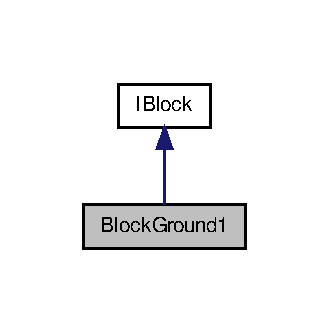
\includegraphics[width=158pt]{class_block_ground1__inherit__graph}
\end{center}
\end{figure}
\subsection*{Public Member Functions}
\begin{DoxyCompactItemize}
\item 
\hypertarget{class_block_ground1_a940fd76a2bb99a72aea37b615250ee5b}{\hyperlink{class_block_ground1_a940fd76a2bb99a72aea37b615250ee5b}{Block\-Ground1} ()}\label{class_block_ground1_a940fd76a2bb99a72aea37b615250ee5b}

\begin{DoxyCompactList}\small\item\em Default constructor. \end{DoxyCompactList}\item 
\hypertarget{class_block_ground1_add8a3546291782546822d80ba08cccba}{virtual \hyperlink{class_block_ground1_add8a3546291782546822d80ba08cccba}{$\sim$\-Block\-Ground1} ()}\label{class_block_ground1_add8a3546291782546822d80ba08cccba}

\begin{DoxyCompactList}\small\item\em Default destructor. \end{DoxyCompactList}\item 
sf\-::\-Texture $\ast$ \hyperlink{class_block_ground1_ae33602300cd0a84d94ce74a1130c77b6}{get\-Texture} ()
\begin{DoxyCompactList}\small\item\em Return the texture of the block. \end{DoxyCompactList}\item 
sf\-::\-Sprite $\ast$ \hyperlink{class_block_ground1_a1764bea828301fadfb0c9a11d43201f7}{get\-Sprite} ()
\begin{DoxyCompactList}\small\item\em Return the sprite of the block. \end{DoxyCompactList}\end{DoxyCompactItemize}
\subsection*{Private Attributes}
\begin{DoxyCompactItemize}
\item 
\hypertarget{class_block_ground1_ab0eaa3f28c57836cbb9bf7232df4146a}{sf\-::\-Texture $\ast$ \hyperlink{class_block_ground1_ab0eaa3f28c57836cbb9bf7232df4146a}{m\-\_\-texture}}\label{class_block_ground1_ab0eaa3f28c57836cbb9bf7232df4146a}

\begin{DoxyCompactList}\small\item\em The texture of the block. \end{DoxyCompactList}\item 
\hypertarget{class_block_ground1_a532dd8b6f9ae6334adb76a79189d18f4}{sf\-::\-Sprite $\ast$ \hyperlink{class_block_ground1_a532dd8b6f9ae6334adb76a79189d18f4}{m\-\_\-sprite}}\label{class_block_ground1_a532dd8b6f9ae6334adb76a79189d18f4}

\begin{DoxyCompactList}\small\item\em The sprite of the block. \end{DoxyCompactList}\end{DoxyCompactItemize}


\subsection{Detailed Description}
A concrete block that implements \hyperlink{class_i_block}{I\-Block}. 

\begin{DoxyAuthor}{Author}
Adrien Bodineau and Alexandre Gomes 
\end{DoxyAuthor}
\begin{DoxyVersion}{Version}
1.\-0 
\end{DoxyVersion}


\subsection{Member Function Documentation}
\hypertarget{class_block_ground1_a1764bea828301fadfb0c9a11d43201f7}{\index{Block\-Ground1@{Block\-Ground1}!get\-Sprite@{get\-Sprite}}
\index{get\-Sprite@{get\-Sprite}!BlockGround1@{Block\-Ground1}}
\subsubsection[{get\-Sprite}]{\setlength{\rightskip}{0pt plus 5cm}sf\-::\-Sprite $\ast$ Block\-Ground1\-::get\-Sprite (
\begin{DoxyParamCaption}
\item[{void}]{}
\end{DoxyParamCaption}
)\hspace{0.3cm}{\ttfamily [virtual]}}}\label{class_block_ground1_a1764bea828301fadfb0c9a11d43201f7}


Return the sprite of the block. 

\begin{DoxyReturn}{Returns}
The sprite of the block 
\end{DoxyReturn}


Implements \hyperlink{class_i_block_a76ae337b47bb084b2c143a24fdc47093}{I\-Block}.

\hypertarget{class_block_ground1_ae33602300cd0a84d94ce74a1130c77b6}{\index{Block\-Ground1@{Block\-Ground1}!get\-Texture@{get\-Texture}}
\index{get\-Texture@{get\-Texture}!BlockGround1@{Block\-Ground1}}
\subsubsection[{get\-Texture}]{\setlength{\rightskip}{0pt plus 5cm}sf\-::\-Texture $\ast$ Block\-Ground1\-::get\-Texture (
\begin{DoxyParamCaption}
{}
\end{DoxyParamCaption}
)\hspace{0.3cm}{\ttfamily [virtual]}}}\label{class_block_ground1_ae33602300cd0a84d94ce74a1130c77b6}


Return the texture of the block. 

\begin{DoxyReturn}{Returns}
The texture of the block 
\end{DoxyReturn}


Implements \hyperlink{class_i_block_ac789384b5d6c070c4f4c6a9c65906826}{I\-Block}.


\hypertarget{class_block_ground2}{\section{Block\-Ground2 Class Reference}
\label{class_block_ground2}\index{Block\-Ground2@{Block\-Ground2}}
}


Another concrete block that implements \hyperlink{class_i_block}{I\-Block}.  




Inheritance diagram for Block\-Ground2\-:\nopagebreak
\begin{figure}[H]
\begin{center}
\leavevmode
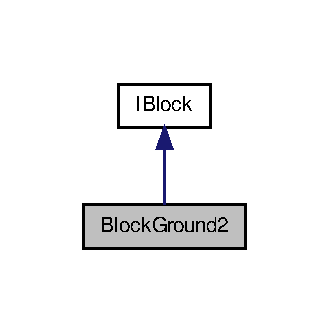
\includegraphics[width=158pt]{class_block_ground2__inherit__graph}
\end{center}
\end{figure}
\subsection*{Public Member Functions}
\begin{DoxyCompactItemize}
\item 
\hypertarget{class_block_ground2_a75fe2a7e690505ea8be19912ecba70b0}{\hyperlink{class_block_ground2_a75fe2a7e690505ea8be19912ecba70b0}{Block\-Ground2} ()}\label{class_block_ground2_a75fe2a7e690505ea8be19912ecba70b0}

\begin{DoxyCompactList}\small\item\em Default constructor. \end{DoxyCompactList}\item 
\hypertarget{class_block_ground2_a1aaf60318df2772a7b073dd15bc15759}{virtual \hyperlink{class_block_ground2_a1aaf60318df2772a7b073dd15bc15759}{$\sim$\-Block\-Ground2} ()}\label{class_block_ground2_a1aaf60318df2772a7b073dd15bc15759}

\begin{DoxyCompactList}\small\item\em Default destructor. \end{DoxyCompactList}\item 
sf\-::\-Texture $\ast$ \hyperlink{class_block_ground2_a97ccf6ca4bbd7d0d45e4fb8550374bf7}{get\-Texture} ()
\begin{DoxyCompactList}\small\item\em Return the texture of the block. \end{DoxyCompactList}\item 
sf\-::\-Sprite $\ast$ \hyperlink{class_block_ground2_aa50914561a51632ac1ad389808e01a43}{get\-Sprite} ()
\begin{DoxyCompactList}\small\item\em Return the sprite of the block. \end{DoxyCompactList}\end{DoxyCompactItemize}
\subsection*{Private Attributes}
\begin{DoxyCompactItemize}
\item 
\hypertarget{class_block_ground2_a66cd8e1758c33a55c95155400b66c279}{sf\-::\-Texture $\ast$ \hyperlink{class_block_ground2_a66cd8e1758c33a55c95155400b66c279}{m\-\_\-texture}}\label{class_block_ground2_a66cd8e1758c33a55c95155400b66c279}

\begin{DoxyCompactList}\small\item\em The texture of the block. \end{DoxyCompactList}\item 
\hypertarget{class_block_ground2_a1e2eaf4d95a0a63062f48b743145b291}{sf\-::\-Sprite $\ast$ \hyperlink{class_block_ground2_a1e2eaf4d95a0a63062f48b743145b291}{m\-\_\-sprite}}\label{class_block_ground2_a1e2eaf4d95a0a63062f48b743145b291}

\begin{DoxyCompactList}\small\item\em The sprite of the block. \end{DoxyCompactList}\end{DoxyCompactItemize}


\subsection{Detailed Description}
Another concrete block that implements \hyperlink{class_i_block}{I\-Block}. 

\begin{DoxyAuthor}{Author}
Adrien Bodineau and Alexandre Gomes 
\end{DoxyAuthor}
\begin{DoxyVersion}{Version}
1.\-0 
\end{DoxyVersion}


\subsection{Member Function Documentation}
\hypertarget{class_block_ground2_aa50914561a51632ac1ad389808e01a43}{\index{Block\-Ground2@{Block\-Ground2}!get\-Sprite@{get\-Sprite}}
\index{get\-Sprite@{get\-Sprite}!BlockGround2@{Block\-Ground2}}
\subsubsection[{get\-Sprite}]{\setlength{\rightskip}{0pt plus 5cm}sf\-::\-Sprite $\ast$ Block\-Ground2\-::get\-Sprite (
\begin{DoxyParamCaption}
\item[{void}]{}
\end{DoxyParamCaption}
)\hspace{0.3cm}{\ttfamily [virtual]}}}\label{class_block_ground2_aa50914561a51632ac1ad389808e01a43}


Return the sprite of the block. 

\begin{DoxyReturn}{Returns}
The sprite of the block 
\end{DoxyReturn}


Implements \hyperlink{class_i_block_a76ae337b47bb084b2c143a24fdc47093}{I\-Block}.

\hypertarget{class_block_ground2_a97ccf6ca4bbd7d0d45e4fb8550374bf7}{\index{Block\-Ground2@{Block\-Ground2}!get\-Texture@{get\-Texture}}
\index{get\-Texture@{get\-Texture}!BlockGround2@{Block\-Ground2}}
\subsubsection[{get\-Texture}]{\setlength{\rightskip}{0pt plus 5cm}sf\-::\-Texture $\ast$ Block\-Ground2\-::get\-Texture (
\begin{DoxyParamCaption}
{}
\end{DoxyParamCaption}
)\hspace{0.3cm}{\ttfamily [virtual]}}}\label{class_block_ground2_a97ccf6ca4bbd7d0d45e4fb8550374bf7}


Return the texture of the block. 

\begin{DoxyReturn}{Returns}
The texture of the block 
\end{DoxyReturn}


Implements \hyperlink{class_i_block_ac789384b5d6c070c4f4c6a9c65906826}{I\-Block}.


\hypertarget{class_block_ground3}{\section{Block\-Ground3 Class Reference}
\label{class_block_ground3}\index{Block\-Ground3@{Block\-Ground3}}
}


Another concrete block that implements \hyperlink{class_i_block}{I\-Block}.  




Inheritance diagram for Block\-Ground3\-:\nopagebreak
\begin{figure}[H]
\begin{center}
\leavevmode
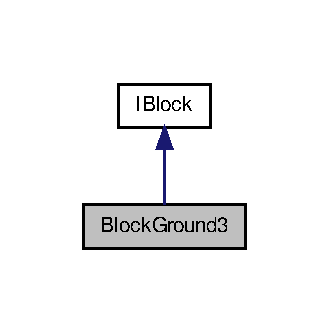
\includegraphics[width=158pt]{class_block_ground3__inherit__graph}
\end{center}
\end{figure}
\subsection*{Public Member Functions}
\begin{DoxyCompactItemize}
\item 
\hypertarget{class_block_ground3_a9511db962f8bafe08244b67403be8c9c}{\hyperlink{class_block_ground3_a9511db962f8bafe08244b67403be8c9c}{Block\-Ground3} ()}\label{class_block_ground3_a9511db962f8bafe08244b67403be8c9c}

\begin{DoxyCompactList}\small\item\em Default constructor. \end{DoxyCompactList}\item 
\hypertarget{class_block_ground3_a35dfc1c85cb0a14e7dab32de4b26dfd8}{virtual \hyperlink{class_block_ground3_a35dfc1c85cb0a14e7dab32de4b26dfd8}{$\sim$\-Block\-Ground3} ()}\label{class_block_ground3_a35dfc1c85cb0a14e7dab32de4b26dfd8}

\begin{DoxyCompactList}\small\item\em Default destructor. \end{DoxyCompactList}\item 
sf\-::\-Texture $\ast$ \hyperlink{class_block_ground3_a356871f712e64b3f9e7efb4075509c40}{get\-Texture} ()
\begin{DoxyCompactList}\small\item\em Return the texture of the block. \end{DoxyCompactList}\item 
sf\-::\-Sprite $\ast$ \hyperlink{class_block_ground3_a55747e1cbcdae3df63da4bacd9eb7d17}{get\-Sprite} ()
\begin{DoxyCompactList}\small\item\em Return the sprite of the block. \end{DoxyCompactList}\end{DoxyCompactItemize}
\subsection*{Private Attributes}
\begin{DoxyCompactItemize}
\item 
\hypertarget{class_block_ground3_a889376a50b100d53ee9b382b06d5bc58}{sf\-::\-Texture $\ast$ \hyperlink{class_block_ground3_a889376a50b100d53ee9b382b06d5bc58}{m\-\_\-texture}}\label{class_block_ground3_a889376a50b100d53ee9b382b06d5bc58}

\begin{DoxyCompactList}\small\item\em The texture of the block. \end{DoxyCompactList}\item 
\hypertarget{class_block_ground3_ac667bb48dd7a1e44efd6a9267367e09f}{sf\-::\-Sprite $\ast$ \hyperlink{class_block_ground3_ac667bb48dd7a1e44efd6a9267367e09f}{m\-\_\-sprite}}\label{class_block_ground3_ac667bb48dd7a1e44efd6a9267367e09f}

\begin{DoxyCompactList}\small\item\em The sprite of the block. \end{DoxyCompactList}\end{DoxyCompactItemize}


\subsection{Detailed Description}
Another concrete block that implements \hyperlink{class_i_block}{I\-Block}. 

\begin{DoxyAuthor}{Author}
Adrien Bodineau and Alexandre Gomes 
\end{DoxyAuthor}
\begin{DoxyVersion}{Version}
1.\-0 
\end{DoxyVersion}


\subsection{Member Function Documentation}
\hypertarget{class_block_ground3_a55747e1cbcdae3df63da4bacd9eb7d17}{\index{Block\-Ground3@{Block\-Ground3}!get\-Sprite@{get\-Sprite}}
\index{get\-Sprite@{get\-Sprite}!BlockGround3@{Block\-Ground3}}
\subsubsection[{get\-Sprite}]{\setlength{\rightskip}{0pt plus 5cm}sf\-::\-Sprite $\ast$ Block\-Ground3\-::get\-Sprite (
\begin{DoxyParamCaption}
\item[{void}]{}
\end{DoxyParamCaption}
)\hspace{0.3cm}{\ttfamily [virtual]}}}\label{class_block_ground3_a55747e1cbcdae3df63da4bacd9eb7d17}


Return the sprite of the block. 

\begin{DoxyReturn}{Returns}
The sprite of the block 
\end{DoxyReturn}


Implements \hyperlink{class_i_block_a76ae337b47bb084b2c143a24fdc47093}{I\-Block}.

\hypertarget{class_block_ground3_a356871f712e64b3f9e7efb4075509c40}{\index{Block\-Ground3@{Block\-Ground3}!get\-Texture@{get\-Texture}}
\index{get\-Texture@{get\-Texture}!BlockGround3@{Block\-Ground3}}
\subsubsection[{get\-Texture}]{\setlength{\rightskip}{0pt plus 5cm}sf\-::\-Texture $\ast$ Block\-Ground3\-::get\-Texture (
\begin{DoxyParamCaption}
{}
\end{DoxyParamCaption}
)\hspace{0.3cm}{\ttfamily [virtual]}}}\label{class_block_ground3_a356871f712e64b3f9e7efb4075509c40}


Return the texture of the block. 

\begin{DoxyReturn}{Returns}
The texture of the block 
\end{DoxyReturn}


Implements \hyperlink{class_i_block_ac789384b5d6c070c4f4c6a9c65906826}{I\-Block}.


\hypertarget{class_cape}{\section{Cape Class Reference}
\label{class_cape}\index{Cape@{Cape}}
}


\hyperlink{class_cape}{Cape} upgrade.  




Inheritance diagram for Cape\-:\nopagebreak
\begin{figure}[H]
\begin{center}
\leavevmode
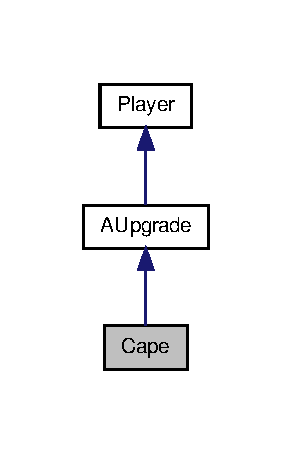
\includegraphics[width=140pt]{class_cape__inherit__graph}
\end{center}
\end{figure}
\subsection*{Public Member Functions}
\begin{DoxyCompactItemize}
\item 
\hyperlink{class_cape_a457e670cb99edbb4590b619b56b04d62}{Cape} (\hyperlink{class_player}{Player} $\ast$character, int pos\-X, int pos\-Y)
\begin{DoxyCompactList}\small\item\em Default constructor. \end{DoxyCompactList}\item 
\hypertarget{class_cape_acd7ada8ed23427dc0ccecde8b400eef9}{virtual \hyperlink{class_cape_acd7ada8ed23427dc0ccecde8b400eef9}{$\sim$\-Cape} ()}\label{class_cape_acd7ada8ed23427dc0ccecde8b400eef9}

\begin{DoxyCompactList}\small\item\em Default destructor. \end{DoxyCompactList}\item 
virtual int \hyperlink{class_cape_a2b563a9b4bd336530dfe01585123a087}{get\-Jump\-Speed} ()
\begin{DoxyCompactList}\small\item\em Get the jumping speed value. \end{DoxyCompactList}\item 
virtual int \hyperlink{class_cape_ac2a629b66fc5b2678ebf294523b53799}{get\-Jump\-Height} ()
\begin{DoxyCompactList}\small\item\em Get the jumping height value. \end{DoxyCompactList}\item 
virtual int \hyperlink{class_cape_addd1a0fc11b71a36950cf8d9516b6869}{get\-Speed} ()
\begin{DoxyCompactList}\small\item\em Get the speed value. \end{DoxyCompactList}\end{DoxyCompactItemize}
\subsection*{Additional Inherited Members}


\subsection{Detailed Description}
\hyperlink{class_cape}{Cape} upgrade. 

\begin{DoxyAuthor}{Author}
Adrien Bodineau and Alexandre Gomes 
\end{DoxyAuthor}
\begin{DoxyVersion}{Version}
1.\-0 
\end{DoxyVersion}


\subsection{Constructor \& Destructor Documentation}
\hypertarget{class_cape_a457e670cb99edbb4590b619b56b04d62}{\index{Cape@{Cape}!Cape@{Cape}}
\index{Cape@{Cape}!Cape@{Cape}}
\subsubsection[{Cape}]{\setlength{\rightskip}{0pt plus 5cm}Cape\-::\-Cape (
\begin{DoxyParamCaption}
\item[{{\bf Player} $\ast$}]{character, }
\item[{int}]{pos\-X, }
\item[{int}]{pos\-Y}
\end{DoxyParamCaption}
)}}\label{class_cape_a457e670cb99edbb4590b619b56b04d62}


Default constructor. 


\begin{DoxyParams}{Parameters}
{\em character} & Decorated character \\
\hline
{\em pos\-X} & Position x \\
\hline
{\em pos\-Y} & Position y \\
\hline
\end{DoxyParams}


\subsection{Member Function Documentation}
\hypertarget{class_cape_ac2a629b66fc5b2678ebf294523b53799}{\index{Cape@{Cape}!get\-Jump\-Height@{get\-Jump\-Height}}
\index{get\-Jump\-Height@{get\-Jump\-Height}!Cape@{Cape}}
\subsubsection[{get\-Jump\-Height}]{\setlength{\rightskip}{0pt plus 5cm}int Cape\-::get\-Jump\-Height (
\begin{DoxyParamCaption}
{}
\end{DoxyParamCaption}
)\hspace{0.3cm}{\ttfamily [virtual]}}}\label{class_cape_ac2a629b66fc5b2678ebf294523b53799}


Get the jumping height value. 

\begin{DoxyReturn}{Returns}
Jumping height value 
\end{DoxyReturn}


Reimplemented from \hyperlink{class_player_a4df8845cc35f7ef2d8aefbeffb141aed}{Player}.

\hypertarget{class_cape_a2b563a9b4bd336530dfe01585123a087}{\index{Cape@{Cape}!get\-Jump\-Speed@{get\-Jump\-Speed}}
\index{get\-Jump\-Speed@{get\-Jump\-Speed}!Cape@{Cape}}
\subsubsection[{get\-Jump\-Speed}]{\setlength{\rightskip}{0pt plus 5cm}int Cape\-::get\-Jump\-Speed (
\begin{DoxyParamCaption}
{}
\end{DoxyParamCaption}
)\hspace{0.3cm}{\ttfamily [virtual]}}}\label{class_cape_a2b563a9b4bd336530dfe01585123a087}


Get the jumping speed value. 

\begin{DoxyReturn}{Returns}
Jump speed value 
\end{DoxyReturn}


Reimplemented from \hyperlink{class_player_a95676c9d2da2c6e778aa8558c5e5fa80}{Player}.

\hypertarget{class_cape_addd1a0fc11b71a36950cf8d9516b6869}{\index{Cape@{Cape}!get\-Speed@{get\-Speed}}
\index{get\-Speed@{get\-Speed}!Cape@{Cape}}
\subsubsection[{get\-Speed}]{\setlength{\rightskip}{0pt plus 5cm}int Cape\-::get\-Speed (
\begin{DoxyParamCaption}
{}
\end{DoxyParamCaption}
)\hspace{0.3cm}{\ttfamily [virtual]}}}\label{class_cape_addd1a0fc11b71a36950cf8d9516b6869}


Get the speed value. 

\begin{DoxyReturn}{Returns}
Speed value 
\end{DoxyReturn}


Reimplemented from \hyperlink{class_player_a5755be9818f6f911d9494e4948d8c483}{Player}.


\hypertarget{class_concrete_factory}{\section{Concrete\-Factory Class Reference}
\label{class_concrete_factory}\index{Concrete\-Factory@{Concrete\-Factory}}
}


A concrete factory to create blocks.  




Inheritance diagram for Concrete\-Factory\-:\nopagebreak
\begin{figure}[H]
\begin{center}
\leavevmode
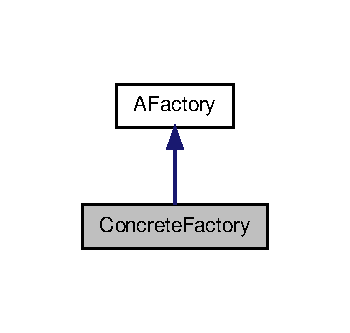
\includegraphics[width=168pt]{class_concrete_factory__inherit__graph}
\end{center}
\end{figure}
\subsection*{Public Member Functions}
\begin{DoxyCompactItemize}
\item 
\hypertarget{class_concrete_factory_a3168082099002e3a6edf4c8cd49847aa}{\hyperlink{class_concrete_factory_a3168082099002e3a6edf4c8cd49847aa}{Concrete\-Factory} ()}\label{class_concrete_factory_a3168082099002e3a6edf4c8cd49847aa}

\begin{DoxyCompactList}\small\item\em Default constructor. \end{DoxyCompactList}\item 
\hypertarget{class_concrete_factory_a9f5ffcdb2424b62151526a4d0cd39a55}{\hyperlink{class_concrete_factory_a9f5ffcdb2424b62151526a4d0cd39a55}{$\sim$\-Concrete\-Factory} ()}\label{class_concrete_factory_a9f5ffcdb2424b62151526a4d0cd39a55}

\begin{DoxyCompactList}\small\item\em Default destructor. \end{DoxyCompactList}\item 
virtual \hyperlink{class_i_block}{I\-Block} $\ast$ \hyperlink{class_concrete_factory_a74d4adfe19116f2fbc31f1c3b745a297}{build} (char s)
\begin{DoxyCompactList}\small\item\em Create a block according to the given character. \end{DoxyCompactList}\end{DoxyCompactItemize}
\subsection*{Additional Inherited Members}


\subsection{Detailed Description}
A concrete factory to create blocks. 

\begin{DoxyAuthor}{Author}
Adrien Bodineau and Alexandre Gomes 
\end{DoxyAuthor}
\begin{DoxyVersion}{Version}
1.\-0 
\end{DoxyVersion}


\subsection{Member Function Documentation}
\hypertarget{class_concrete_factory_a74d4adfe19116f2fbc31f1c3b745a297}{\index{Concrete\-Factory@{Concrete\-Factory}!build@{build}}
\index{build@{build}!ConcreteFactory@{Concrete\-Factory}}
\subsubsection[{build}]{\setlength{\rightskip}{0pt plus 5cm}{\bf I\-Block} $\ast$ Concrete\-Factory\-::build (
\begin{DoxyParamCaption}
\item[{char}]{s}
\end{DoxyParamCaption}
)\hspace{0.3cm}{\ttfamily [virtual]}}}\label{class_concrete_factory_a74d4adfe19116f2fbc31f1c3b745a297}


Create a block according to the given character. 


\begin{DoxyParams}{Parameters}
{\em s} & A char that indicate the block to construct \\
\hline
\end{DoxyParams}
\begin{DoxyReturn}{Returns}
The block constructed 
\end{DoxyReturn}


Implements \hyperlink{class_a_factory_adec2bf9f81dbf37ef727bcfb43403867}{A\-Factory}.


\hypertarget{class_game_manager}{\section{Game\-Manager Class Reference}
\label{class_game_manager}\index{Game\-Manager@{Game\-Manager}}
}


Provide an instance to manage the game.  


\subsection*{Public Member Functions}
\begin{DoxyCompactItemize}
\item 
\hypertarget{class_game_manager_acdc9d0af34329c0a5bf6f0949727a413}{virtual \hyperlink{class_game_manager_acdc9d0af34329c0a5bf6f0949727a413}{$\sim$\-Game\-Manager} (void)}\label{class_game_manager_acdc9d0af34329c0a5bf6f0949727a413}

\begin{DoxyCompactList}\small\item\em The default destructor. \end{DoxyCompactList}\item 
\hypertarget{class_game_manager_a30c2267cebe64ca70ec49c8560ceaf70}{void \hyperlink{class_game_manager_a30c2267cebe64ca70ec49c8560ceaf70}{action} (void)}\label{class_game_manager_a30c2267cebe64ca70ec49c8560ceaf70}

\begin{DoxyCompactList}\small\item\em Set up the parameters and run the game loop. \end{DoxyCompactList}\item 
\hypertarget{class_game_manager_a503f08e6803a70c65c324a88078da558}{void \hyperlink{class_game_manager_a503f08e6803a70c65c324a88078da558}{update} (void)}\label{class_game_manager_a503f08e6803a70c65c324a88078da558}

\begin{DoxyCompactList}\small\item\em Update the data of the game. \end{DoxyCompactList}\item 
\hypertarget{class_game_manager_acaf23b5999e093f95350b377930709f2}{void \hyperlink{class_game_manager_acaf23b5999e093f95350b377930709f2}{draw} (void)}\label{class_game_manager_acaf23b5999e093f95350b377930709f2}

\begin{DoxyCompactList}\small\item\em Draw the elements of the game on the screen. \end{DoxyCompactList}\item 
\hypertarget{class_game_manager_afc42f60e3bc2b27d2c1c97db4f0d0f5d}{void \hyperlink{class_game_manager_afc42f60e3bc2b27d2c1c97db4f0d0f5d}{collision\-R} (void)}\label{class_game_manager_afc42f60e3bc2b27d2c1c97db4f0d0f5d}

\begin{DoxyCompactList}\small\item\em Check if the player is colliding with an object on his right. \end{DoxyCompactList}\item 
\hypertarget{class_game_manager_abafc8b11a6ea10a83b1e0f218fd5133d}{void \hyperlink{class_game_manager_abafc8b11a6ea10a83b1e0f218fd5133d}{collision\-L} (void)}\label{class_game_manager_abafc8b11a6ea10a83b1e0f218fd5133d}

\begin{DoxyCompactList}\small\item\em Check if the player is colliding with an object on his left. \end{DoxyCompactList}\item 
\hypertarget{class_game_manager_a7aaec061aabf7f4e5ba8fed7b7415b84}{void \hyperlink{class_game_manager_a7aaec061aabf7f4e5ba8fed7b7415b84}{collision\-T} (void)}\label{class_game_manager_a7aaec061aabf7f4e5ba8fed7b7415b84}

\begin{DoxyCompactList}\small\item\em Check if the player is colliding with an object on his top. \end{DoxyCompactList}\item 
\hypertarget{class_game_manager_a6848d5f06fd715a809179df02139bd3a}{void \hyperlink{class_game_manager_a6848d5f06fd715a809179df02139bd3a}{collision\-G} (void)}\label{class_game_manager_a6848d5f06fd715a809179df02139bd3a}

\begin{DoxyCompactList}\small\item\em Check if the player is on the ground. \end{DoxyCompactList}\end{DoxyCompactItemize}
\subsection*{Static Public Member Functions}
\begin{DoxyCompactItemize}
\item 
static \hyperlink{class_game_manager}{Game\-Manager} $\ast$ \hyperlink{class_game_manager_aee0b0f084c86ece89f9f49353ef75e6e}{get\-Instance} (void)
\begin{DoxyCompactList}\small\item\em Give the instance of the class, and create it if it's required. \end{DoxyCompactList}\end{DoxyCompactItemize}
\subsection*{Private Member Functions}
\begin{DoxyCompactItemize}
\item 
\hyperlink{class_game_manager_ad7179b31cffea9c6f7d2ea02ce4f7f86}{Game\-Manager} (int width, int height, std\-::string const \&title)
\begin{DoxyCompactList}\small\item\em Private constructor of the class. \end{DoxyCompactList}\end{DoxyCompactItemize}
\subsection*{Private Attributes}
\begin{DoxyCompactItemize}
\item 
\hypertarget{class_game_manager_a1b279dfcddfd51a081714cb7d638a47d}{\hyperlink{class_player}{Player} $\ast$ \hyperlink{class_game_manager_a1b279dfcddfd51a081714cb7d638a47d}{m\-\_\-player}}\label{class_game_manager_a1b279dfcddfd51a081714cb7d638a47d}

\begin{DoxyCompactList}\small\item\em Pointer on the player. \end{DoxyCompactList}\item 
\hypertarget{class_game_manager_aad6835720aa63bec36cf93a13f7ff9ec}{sf\-::\-Render\-Window $\ast$ \hyperlink{class_game_manager_aad6835720aa63bec36cf93a13f7ff9ec}{m\-\_\-screen}}\label{class_game_manager_aad6835720aa63bec36cf93a13f7ff9ec}

\begin{DoxyCompactList}\small\item\em Pointer on the screen. \end{DoxyCompactList}\item 
\hypertarget{class_game_manager_a655c1cad03fda61336ed812bdf641a82}{sf\-::\-View $\ast$ \hyperlink{class_game_manager_a655c1cad03fda61336ed812bdf641a82}{m\-\_\-view}}\label{class_game_manager_a655c1cad03fda61336ed812bdf641a82}

\begin{DoxyCompactList}\small\item\em Pointer on the view (2\-D camera) \end{DoxyCompactList}\item 
\hypertarget{class_game_manager_ab7cdbdc9d701e4e2c57319946b18f75c}{\hyperlink{class_i_level}{I\-Level} $\ast$ \hyperlink{class_game_manager_ab7cdbdc9d701e4e2c57319946b18f75c}{m\-\_\-level}}\label{class_game_manager_ab7cdbdc9d701e4e2c57319946b18f75c}

\begin{DoxyCompactList}\small\item\em Pointer on the level. \end{DoxyCompactList}\item 
\hypertarget{class_game_manager_a47f464b9a9dfbb6b29425d067652e06e}{char $\ast$ \hyperlink{class_game_manager_a47f464b9a9dfbb6b29425d067652e06e}{m\-\_\-col\-G}}\label{class_game_manager_a47f464b9a9dfbb6b29425d067652e06e}

\begin{DoxyCompactList}\small\item\em Pointer to check the ground collision. \end{DoxyCompactList}\item 
\hypertarget{class_game_manager_a585bc82f812508cf7e1fcaa61d16b4b5}{char $\ast$ \hyperlink{class_game_manager_a585bc82f812508cf7e1fcaa61d16b4b5}{m\-\_\-col\-L}}\label{class_game_manager_a585bc82f812508cf7e1fcaa61d16b4b5}

\begin{DoxyCompactList}\small\item\em Pointer to check the left collision. \end{DoxyCompactList}\item 
\hypertarget{class_game_manager_a453919435a19f51aac53370ab1761dd5}{char $\ast$ \hyperlink{class_game_manager_a453919435a19f51aac53370ab1761dd5}{m\-\_\-col\-T}}\label{class_game_manager_a453919435a19f51aac53370ab1761dd5}

\begin{DoxyCompactList}\small\item\em Pointer to check the top collision. \end{DoxyCompactList}\item 
\hypertarget{class_game_manager_a0a9aa8ed8be6c9f8ff3c61ab72948bd9}{char $\ast$ \hyperlink{class_game_manager_a0a9aa8ed8be6c9f8ff3c61ab72948bd9}{m\-\_\-col\-R}}\label{class_game_manager_a0a9aa8ed8be6c9f8ff3c61ab72948bd9}

\begin{DoxyCompactList}\small\item\em Pointer to check the right collision. \end{DoxyCompactList}\item 
\hypertarget{class_game_manager_aef88fa7485663c973fe47350894441ee}{bool \hyperlink{class_game_manager_aef88fa7485663c973fe47350894441ee}{m\-\_\-win}}\label{class_game_manager_aef88fa7485663c973fe47350894441ee}

\begin{DoxyCompactList}\small\item\em Boolean to check if the player has won, true if he has, false otherwise. \end{DoxyCompactList}\item 
\hypertarget{class_game_manager_abd261afcb9a4f75c1a0fa1cd707a7c8f}{bool \hyperlink{class_game_manager_abd261afcb9a4f75c1a0fa1cd707a7c8f}{m\-\_\-lost}}\label{class_game_manager_abd261afcb9a4f75c1a0fa1cd707a7c8f}

\begin{DoxyCompactList}\small\item\em Boolean to check if the player has lost, true if he has, false otherwise. \end{DoxyCompactList}\item 
\hypertarget{class_game_manager_aa9ea92449084ccab8f3a7467b3a56524}{sf\-::\-Music $\ast$ \hyperlink{class_game_manager_aa9ea92449084ccab8f3a7467b3a56524}{m\-\_\-music}}\label{class_game_manager_aa9ea92449084ccab8f3a7467b3a56524}

\begin{DoxyCompactList}\small\item\em Pointer to the music of the current level. \end{DoxyCompactList}\item 
\hypertarget{class_game_manager_ad91a331f6af536db50fe1794c194871d}{sf\-::\-Sound $\ast$ \hyperlink{class_game_manager_ad91a331f6af536db50fe1794c194871d}{m\-\_\-upgrade\-Sound}}\label{class_game_manager_ad91a331f6af536db50fe1794c194871d}

\begin{DoxyCompactList}\small\item\em Pointer to the upgrade sound. \end{DoxyCompactList}\item 
\hypertarget{class_game_manager_a22fb2acccebe7dc6bd893a39ba747a38}{sf\-::\-Sound\-Buffer $\ast$ \hyperlink{class_game_manager_a22fb2acccebe7dc6bd893a39ba747a38}{m\-\_\-upgrade\-Sound\-Buffer}}\label{class_game_manager_a22fb2acccebe7dc6bd893a39ba747a38}

\begin{DoxyCompactList}\small\item\em Pointer to the buffer of the upgrade sound. \end{DoxyCompactList}\item 
\hypertarget{class_game_manager_a56334ff5fbd86615dfb9e03f2edc5248}{sf\-::\-Sound $\ast$ \hyperlink{class_game_manager_a56334ff5fbd86615dfb9e03f2edc5248}{m\-\_\-lost\-Sound}}\label{class_game_manager_a56334ff5fbd86615dfb9e03f2edc5248}

\begin{DoxyCompactList}\small\item\em Pointer to the lost sound. \end{DoxyCompactList}\item 
\hypertarget{class_game_manager_aad51c87666d9a388634cc3cd046114cc}{sf\-::\-Sound\-Buffer $\ast$ \hyperlink{class_game_manager_aad51c87666d9a388634cc3cd046114cc}{m\-\_\-lost\-Sound\-Buffer}}\label{class_game_manager_aad51c87666d9a388634cc3cd046114cc}

\begin{DoxyCompactList}\small\item\em Pointer to the buffer of the lost sound. \end{DoxyCompactList}\item 
\hypertarget{class_game_manager_a587e2e15b42ba0334bfaf344ad9429c7}{sf\-::\-Sound $\ast$ \hyperlink{class_game_manager_a587e2e15b42ba0334bfaf344ad9429c7}{m\-\_\-win\-Sound}}\label{class_game_manager_a587e2e15b42ba0334bfaf344ad9429c7}

\begin{DoxyCompactList}\small\item\em Pointer to the win sound. \end{DoxyCompactList}\item 
\hypertarget{class_game_manager_ab7e281ae47b37721117c0ddf7f9f36e0}{sf\-::\-Sound\-Buffer $\ast$ \hyperlink{class_game_manager_ab7e281ae47b37721117c0ddf7f9f36e0}{m\-\_\-win\-Sound\-Buffer}}\label{class_game_manager_ab7e281ae47b37721117c0ddf7f9f36e0}

\begin{DoxyCompactList}\small\item\em Pointer to the buffer of the win sound. \end{DoxyCompactList}\end{DoxyCompactItemize}
\subsection*{Static Private Attributes}
\begin{DoxyCompactItemize}
\item 
\hypertarget{class_game_manager_a2bf6eac738e0ba23fa7a1d4273954c79}{static \hyperlink{class_game_manager}{Game\-Manager} $\ast$ \hyperlink{class_game_manager_a2bf6eac738e0ba23fa7a1d4273954c79}{m\-\_\-game\-Manager}}\label{class_game_manager_a2bf6eac738e0ba23fa7a1d4273954c79}

\begin{DoxyCompactList}\small\item\em Static pointer on the unique instance of the class. \end{DoxyCompactList}\end{DoxyCompactItemize}


\subsection{Detailed Description}
Provide an instance to manage the game. 

\begin{DoxyAuthor}{Author}
Adrien Bodineau and Alexandre Gomes 
\end{DoxyAuthor}
\begin{DoxyVersion}{Version}
1.\-0 
\end{DoxyVersion}


\subsection{Constructor \& Destructor Documentation}
\hypertarget{class_game_manager_ad7179b31cffea9c6f7d2ea02ce4f7f86}{\index{Game\-Manager@{Game\-Manager}!Game\-Manager@{Game\-Manager}}
\index{Game\-Manager@{Game\-Manager}!GameManager@{Game\-Manager}}
\subsubsection[{Game\-Manager}]{\setlength{\rightskip}{0pt plus 5cm}Game\-Manager\-::\-Game\-Manager (
\begin{DoxyParamCaption}
\item[{int}]{width, }
\item[{int}]{height, }
\item[{std\-::string const \&}]{title}
\end{DoxyParamCaption}
)\hspace{0.3cm}{\ttfamily [private]}}}\label{class_game_manager_ad7179b31cffea9c6f7d2ea02ce4f7f86}


Private constructor of the class. 


\begin{DoxyParams}{Parameters}
{\em width} & An integer representing the width of the screen \\
\hline
{\em height} & An integer representing the height of the screen \\
\hline
{\em title} & A string representing the title of the screen \\
\hline
\end{DoxyParams}


\subsection{Member Function Documentation}
\hypertarget{class_game_manager_aee0b0f084c86ece89f9f49353ef75e6e}{\index{Game\-Manager@{Game\-Manager}!get\-Instance@{get\-Instance}}
\index{get\-Instance@{get\-Instance}!GameManager@{Game\-Manager}}
\subsubsection[{get\-Instance}]{\setlength{\rightskip}{0pt plus 5cm}static {\bf Game\-Manager} $\ast$ Game\-Manager\-::get\-Instance (
\begin{DoxyParamCaption}
\item[{void}]{}
\end{DoxyParamCaption}
)\hspace{0.3cm}{\ttfamily [inline]}, {\ttfamily [static]}}}\label{class_game_manager_aee0b0f084c86ece89f9f49353ef75e6e}


Give the instance of the class, and create it if it's required. 

\begin{DoxyReturn}{Returns}
A pointer on the instance of the class 
\end{DoxyReturn}

\hypertarget{class_i_block}{\section{I\-Block Class Reference}
\label{class_i_block}\index{I\-Block@{I\-Block}}
}


Interface that will be implemented by all the different kinds of blocks.  




Inheritance diagram for I\-Block\-:\nopagebreak
\begin{figure}[H]
\begin{center}
\leavevmode
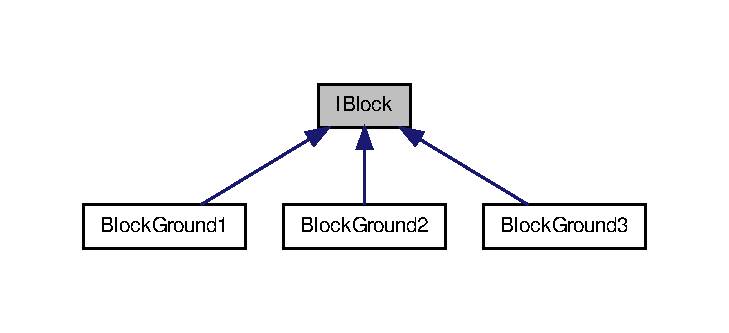
\includegraphics[width=350pt]{class_i_block__inherit__graph}
\end{center}
\end{figure}
\subsection*{Public Member Functions}
\begin{DoxyCompactItemize}
\item 
virtual sf\-::\-Texture $\ast$ \hyperlink{class_i_block_ac789384b5d6c070c4f4c6a9c65906826}{get\-Texture} ()=0
\begin{DoxyCompactList}\small\item\em Return the texture of the block. \end{DoxyCompactList}\item 
virtual sf\-::\-Sprite $\ast$ \hyperlink{class_i_block_a76ae337b47bb084b2c143a24fdc47093}{get\-Sprite} ()=0
\begin{DoxyCompactList}\small\item\em Return the sprite of the block. \end{DoxyCompactList}\end{DoxyCompactItemize}


\subsection{Detailed Description}
Interface that will be implemented by all the different kinds of blocks. 

\begin{DoxyAuthor}{Author}
Adrien Bodineau and Alexandre Gomes 
\end{DoxyAuthor}
\begin{DoxyVersion}{Version}
1.\-0 
\end{DoxyVersion}


\subsection{Member Function Documentation}
\hypertarget{class_i_block_a76ae337b47bb084b2c143a24fdc47093}{\index{I\-Block@{I\-Block}!get\-Sprite@{get\-Sprite}}
\index{get\-Sprite@{get\-Sprite}!IBlock@{I\-Block}}
\subsubsection[{get\-Sprite}]{\setlength{\rightskip}{0pt plus 5cm}sf\-::\-Sprite $\ast$ I\-Block\-::get\-Sprite (
\begin{DoxyParamCaption}
\item[{void}]{}
\end{DoxyParamCaption}
)\hspace{0.3cm}{\ttfamily [pure virtual]}}}\label{class_i_block_a76ae337b47bb084b2c143a24fdc47093}


Return the sprite of the block. 

\begin{DoxyReturn}{Returns}
The sprite of the block 
\end{DoxyReturn}


Implemented in \hyperlink{class_block_ground1_a1764bea828301fadfb0c9a11d43201f7}{Block\-Ground1}, \hyperlink{class_block_ground2_aa50914561a51632ac1ad389808e01a43}{Block\-Ground2}, and \hyperlink{class_block_ground3_a55747e1cbcdae3df63da4bacd9eb7d17}{Block\-Ground3}.

\hypertarget{class_i_block_ac789384b5d6c070c4f4c6a9c65906826}{\index{I\-Block@{I\-Block}!get\-Texture@{get\-Texture}}
\index{get\-Texture@{get\-Texture}!IBlock@{I\-Block}}
\subsubsection[{get\-Texture}]{\setlength{\rightskip}{0pt plus 5cm}sf\-::\-Texture $\ast$ I\-Block\-::get\-Texture (
\begin{DoxyParamCaption}
{}
\end{DoxyParamCaption}
)\hspace{0.3cm}{\ttfamily [pure virtual]}}}\label{class_i_block_ac789384b5d6c070c4f4c6a9c65906826}


Return the texture of the block. 

\begin{DoxyReturn}{Returns}
The texture of the block 
\end{DoxyReturn}


Implemented in \hyperlink{class_block_ground1_ae33602300cd0a84d94ce74a1130c77b6}{Block\-Ground1}, \hyperlink{class_block_ground2_a97ccf6ca4bbd7d0d45e4fb8550374bf7}{Block\-Ground2}, and \hyperlink{class_block_ground3_a356871f712e64b3f9e7efb4075509c40}{Block\-Ground3}.


\hypertarget{class_i_level}{\section{I\-Level Class Reference}
\label{class_i_level}\index{I\-Level@{I\-Level}}
}


Interface that will be implemented by the levels.  




Inheritance diagram for I\-Level\-:\nopagebreak
\begin{figure}[H]
\begin{center}
\leavevmode
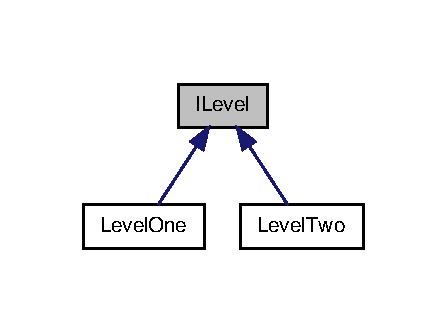
\includegraphics[width=214pt]{class_i_level__inherit__graph}
\end{center}
\end{figure}
\subsection*{Public Member Functions}
\begin{DoxyCompactItemize}
\item 
\hypertarget{class_i_level_a736c3cb25ccf5c3f8a79522eef06351d}{virtual \hyperlink{class_i_level_a736c3cb25ccf5c3f8a79522eef06351d}{$\sim$\-I\-Level} ()}\label{class_i_level_a736c3cb25ccf5c3f8a79522eef06351d}

\begin{DoxyCompactList}\small\item\em Default destructor. \end{DoxyCompactList}\item 
virtual int \hyperlink{class_i_level_a192bb8106e09fb68794711b048ca748d}{get\-Height} (void)=0
\begin{DoxyCompactList}\small\item\em Get the height of the level. \end{DoxyCompactList}\item 
virtual int \hyperlink{class_i_level_a91daa2f5b760da916b348470cd5ed66e}{get\-Width} (void)=0
\begin{DoxyCompactList}\small\item\em Get the width of the level. \end{DoxyCompactList}\item 
virtual void \hyperlink{class_i_level_ae5c21f7cc2cc8757ef50b767d4787138}{load\-Level} (\hyperlink{class_player}{Player} $\ast$player)=0
\begin{DoxyCompactList}\small\item\em Load the level and the player according the tile map. \end{DoxyCompactList}\item 
virtual void \hyperlink{class_i_level_a7e37723d1806e1c137c332fd4b28ba51}{draw\-Level} (sf\-::\-Render\-Window $\ast$screen)=0
\begin{DoxyCompactList}\small\item\em Draw all the elements of the level on the given screen. \end{DoxyCompactList}\item 
virtual std\-::vector\\*
$<$ sf\-::\-Sprite $\ast$ $>$ $\ast$ \hyperlink{class_i_level_a9d3f0ff762fbb04038eac9de4531bc45}{get\-Blocks} ()=0
\begin{DoxyCompactList}\small\item\em Get the blocks of the level. \end{DoxyCompactList}\item 
virtual sf\-::\-Sprite $\ast$ \hyperlink{class_i_level_a458fa2042948a69f5ec6951e77f9459e}{get\-End\-Sprite} (void)=0
\begin{DoxyCompactList}\small\item\em Get the sprite of the end. \end{DoxyCompactList}\item 
virtual \hyperlink{class_i_level}{I\-Level} $\ast$ \hyperlink{class_i_level_a78b187489e43f061cbd990d9ae957178}{get\-Next} (void)=0
\begin{DoxyCompactList}\small\item\em Get the next level. \end{DoxyCompactList}\item 
virtual sf\-::\-Sprite $\ast$ \hyperlink{class_i_level_a63d5e1443bff759199d0eb60b0f1eb1f}{get\-Cape\-Sprite} ()=0
\begin{DoxyCompactList}\small\item\em Get the sprite of the cape. \end{DoxyCompactList}\item 
virtual sf\-::\-Sprite $\ast$ \hyperlink{class_i_level_ac418e1773d0df3be6ddd40091f04689f}{get\-Shoes\-Sprite} ()=0
\begin{DoxyCompactList}\small\item\em Get the sprite of the shoes. \end{DoxyCompactList}\item 
virtual void \hyperlink{class_i_level_a185d4dd983c714a10a2bbdaebae202e6}{remove\-Element} (char target)=0
\begin{DoxyCompactList}\small\item\em Remove an element from the map. \end{DoxyCompactList}\end{DoxyCompactItemize}


\subsection{Detailed Description}
Interface that will be implemented by the levels. 

\begin{DoxyAuthor}{Author}
Adrien Bodineau and Alexandre Gomes 
\end{DoxyAuthor}
\begin{DoxyVersion}{Version}
1.\-0 
\end{DoxyVersion}


\subsection{Member Function Documentation}
\hypertarget{class_i_level_a7e37723d1806e1c137c332fd4b28ba51}{\index{I\-Level@{I\-Level}!draw\-Level@{draw\-Level}}
\index{draw\-Level@{draw\-Level}!ILevel@{I\-Level}}
\subsubsection[{draw\-Level}]{\setlength{\rightskip}{0pt plus 5cm}void I\-Level\-::draw\-Level (
\begin{DoxyParamCaption}
\item[{sf\-::\-Render\-Window $\ast$}]{screen}
\end{DoxyParamCaption}
)\hspace{0.3cm}{\ttfamily [pure virtual]}}}\label{class_i_level_a7e37723d1806e1c137c332fd4b28ba51}


Draw all the elements of the level on the given screen. 


\begin{DoxyParams}{Parameters}
{\em screen} & The screen where the elements will be displayed \\
\hline
\end{DoxyParams}


Implemented in \hyperlink{class_level_one_ac0c5c722d11a026de024ab4a4cbd20ff}{Level\-One}, and \hyperlink{class_level_two_a6fbf138025c013260c7f572b41468a24}{Level\-Two}.

\hypertarget{class_i_level_a9d3f0ff762fbb04038eac9de4531bc45}{\index{I\-Level@{I\-Level}!get\-Blocks@{get\-Blocks}}
\index{get\-Blocks@{get\-Blocks}!ILevel@{I\-Level}}
\subsubsection[{get\-Blocks}]{\setlength{\rightskip}{0pt plus 5cm}std\-::vector$<$ sf\-::\-Sprite $\ast$ $>$ $\ast$ I\-Level\-::get\-Blocks (
\begin{DoxyParamCaption}
\item[{void}]{}
\end{DoxyParamCaption}
)\hspace{0.3cm}{\ttfamily [pure virtual]}}}\label{class_i_level_a9d3f0ff762fbb04038eac9de4531bc45}


Get the blocks of the level. 

\begin{DoxyReturn}{Returns}
A vector with all the elements 
\end{DoxyReturn}


Implemented in \hyperlink{class_level_one_a1037e8727782792343b7374eddd535af}{Level\-One}, and \hyperlink{class_level_two_a412f81d5b2b93ea6690635cc5ce02c8f}{Level\-Two}.

\hypertarget{class_i_level_a63d5e1443bff759199d0eb60b0f1eb1f}{\index{I\-Level@{I\-Level}!get\-Cape\-Sprite@{get\-Cape\-Sprite}}
\index{get\-Cape\-Sprite@{get\-Cape\-Sprite}!ILevel@{I\-Level}}
\subsubsection[{get\-Cape\-Sprite}]{\setlength{\rightskip}{0pt plus 5cm}sf\-::\-Sprite $\ast$ I\-Level\-::get\-Cape\-Sprite (
\begin{DoxyParamCaption}
\item[{void}]{}
\end{DoxyParamCaption}
)\hspace{0.3cm}{\ttfamily [pure virtual]}}}\label{class_i_level_a63d5e1443bff759199d0eb60b0f1eb1f}


Get the sprite of the cape. 

\begin{DoxyReturn}{Returns}
Sprite of the cape 
\end{DoxyReturn}


Implemented in \hyperlink{class_level_one_aa2bb199782d979d50a7143ffb9c3a2a5}{Level\-One}, and \hyperlink{class_level_two_af9e5022cbec0fe1ec6171231374161dd}{Level\-Two}.

\hypertarget{class_i_level_a458fa2042948a69f5ec6951e77f9459e}{\index{I\-Level@{I\-Level}!get\-End\-Sprite@{get\-End\-Sprite}}
\index{get\-End\-Sprite@{get\-End\-Sprite}!ILevel@{I\-Level}}
\subsubsection[{get\-End\-Sprite}]{\setlength{\rightskip}{0pt plus 5cm}sf\-::\-Sprite $\ast$ I\-Level\-::get\-End\-Sprite (
\begin{DoxyParamCaption}
\item[{void}]{}
\end{DoxyParamCaption}
)\hspace{0.3cm}{\ttfamily [pure virtual]}}}\label{class_i_level_a458fa2042948a69f5ec6951e77f9459e}


Get the sprite of the end. 

\begin{DoxyReturn}{Returns}
The sprite of the end 
\end{DoxyReturn}


Implemented in \hyperlink{class_level_one_a2fb4139507f1b0168e8adc3e137d1e94}{Level\-One}, and \hyperlink{class_level_two_a981cce04240b7d5bf4e5dc5b8a212319}{Level\-Two}.

\hypertarget{class_i_level_a192bb8106e09fb68794711b048ca748d}{\index{I\-Level@{I\-Level}!get\-Height@{get\-Height}}
\index{get\-Height@{get\-Height}!ILevel@{I\-Level}}
\subsubsection[{get\-Height}]{\setlength{\rightskip}{0pt plus 5cm}int I\-Level\-::get\-Height (
\begin{DoxyParamCaption}
\item[{void}]{}
\end{DoxyParamCaption}
)\hspace{0.3cm}{\ttfamily [pure virtual]}}}\label{class_i_level_a192bb8106e09fb68794711b048ca748d}


Get the height of the level. 

\begin{DoxyReturn}{Returns}
The height of the level 
\end{DoxyReturn}


Implemented in \hyperlink{class_level_one_ad42ac4352d8559121504d6ff19a76cde}{Level\-One}, and \hyperlink{class_level_two_a8c0c117bce3509249967c408b5e077a4}{Level\-Two}.

\hypertarget{class_i_level_a78b187489e43f061cbd990d9ae957178}{\index{I\-Level@{I\-Level}!get\-Next@{get\-Next}}
\index{get\-Next@{get\-Next}!ILevel@{I\-Level}}
\subsubsection[{get\-Next}]{\setlength{\rightskip}{0pt plus 5cm}{\bf I\-Level} $\ast$ I\-Level\-::get\-Next (
\begin{DoxyParamCaption}
\item[{void}]{}
\end{DoxyParamCaption}
)\hspace{0.3cm}{\ttfamily [pure virtual]}}}\label{class_i_level_a78b187489e43f061cbd990d9ae957178}


Get the next level. 

\begin{DoxyReturn}{Returns}
Next level, N\-U\-L\-L if this is the last level 
\end{DoxyReturn}


Implemented in \hyperlink{class_level_one_a02759e21a744625e01f936e529b0e8f1}{Level\-One}, and \hyperlink{class_level_two_a4f0b0678a51169126fdd0e354ff4fa0e}{Level\-Two}.

\hypertarget{class_i_level_ac418e1773d0df3be6ddd40091f04689f}{\index{I\-Level@{I\-Level}!get\-Shoes\-Sprite@{get\-Shoes\-Sprite}}
\index{get\-Shoes\-Sprite@{get\-Shoes\-Sprite}!ILevel@{I\-Level}}
\subsubsection[{get\-Shoes\-Sprite}]{\setlength{\rightskip}{0pt plus 5cm}sf\-::\-Sprite $\ast$ I\-Level\-::get\-Shoes\-Sprite (
\begin{DoxyParamCaption}
\item[{void}]{}
\end{DoxyParamCaption}
)\hspace{0.3cm}{\ttfamily [pure virtual]}}}\label{class_i_level_ac418e1773d0df3be6ddd40091f04689f}


Get the sprite of the shoes. 

\begin{DoxyReturn}{Returns}
Sprite of the shoes 
\end{DoxyReturn}


Implemented in \hyperlink{class_level_one_ab7b81a5ee8299a900494439e470e0f17}{Level\-One}, and \hyperlink{class_level_two_ae382cc1e788e71eadcef2b5946ee204e}{Level\-Two}.

\hypertarget{class_i_level_a91daa2f5b760da916b348470cd5ed66e}{\index{I\-Level@{I\-Level}!get\-Width@{get\-Width}}
\index{get\-Width@{get\-Width}!ILevel@{I\-Level}}
\subsubsection[{get\-Width}]{\setlength{\rightskip}{0pt plus 5cm}int I\-Level\-::get\-Width (
\begin{DoxyParamCaption}
\item[{void}]{}
\end{DoxyParamCaption}
)\hspace{0.3cm}{\ttfamily [pure virtual]}}}\label{class_i_level_a91daa2f5b760da916b348470cd5ed66e}


Get the width of the level. 

\begin{DoxyReturn}{Returns}
The width of the level 
\end{DoxyReturn}


Implemented in \hyperlink{class_level_one_acc6a1535bc43ee0cd38e9ae688d71f41}{Level\-One}, and \hyperlink{class_level_two_a8b5c8339077204363fc53e861710ca5c}{Level\-Two}.

\hypertarget{class_i_level_ae5c21f7cc2cc8757ef50b767d4787138}{\index{I\-Level@{I\-Level}!load\-Level@{load\-Level}}
\index{load\-Level@{load\-Level}!ILevel@{I\-Level}}
\subsubsection[{load\-Level}]{\setlength{\rightskip}{0pt plus 5cm}void I\-Level\-::load\-Level (
\begin{DoxyParamCaption}
\item[{{\bf Player} $\ast$}]{player}
\end{DoxyParamCaption}
)\hspace{0.3cm}{\ttfamily [pure virtual]}}}\label{class_i_level_ae5c21f7cc2cc8757ef50b767d4787138}


Load the level and the player according the tile map. 


\begin{DoxyParams}{Parameters}
{\em player} & The pointer to the player, so the method can set his position \\
\hline
\end{DoxyParams}


Implemented in \hyperlink{class_level_one_a072a98e693b35e9d8bafc7ae78966a86}{Level\-One}, and \hyperlink{class_level_two_a71138ffe84dee9ed856a0328f3c72411}{Level\-Two}.

\hypertarget{class_i_level_a185d4dd983c714a10a2bbdaebae202e6}{\index{I\-Level@{I\-Level}!remove\-Element@{remove\-Element}}
\index{remove\-Element@{remove\-Element}!ILevel@{I\-Level}}
\subsubsection[{remove\-Element}]{\setlength{\rightskip}{0pt plus 5cm}void I\-Level\-::remove\-Element (
\begin{DoxyParamCaption}
\item[{char}]{target}
\end{DoxyParamCaption}
)\hspace{0.3cm}{\ttfamily [pure virtual]}}}\label{class_i_level_a185d4dd983c714a10a2bbdaebae202e6}


Remove an element from the map. 


\begin{DoxyParams}{Parameters}
{\em target} & Character representing the element to remove \\
\hline
\end{DoxyParams}


Implemented in \hyperlink{class_level_one_a601628107a9810e5c323dc994d7c07ec}{Level\-One}, and \hyperlink{class_level_two_a87ad50b6da9f82ecf602c789d354acae}{Level\-Two}.


\hypertarget{class_level_one}{\section{Level\-One Class Reference}
\label{class_level_one}\index{Level\-One@{Level\-One}}
}


Implements the first level of the game.  




Inheritance diagram for Level\-One\-:\nopagebreak
\begin{figure}[H]
\begin{center}
\leavevmode
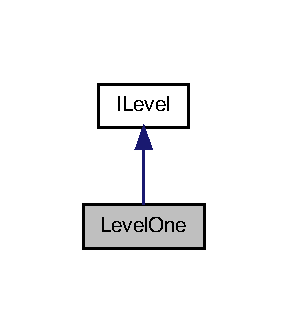
\includegraphics[width=138pt]{class_level_one__inherit__graph}
\end{center}
\end{figure}
\subsection*{Public Member Functions}
\begin{DoxyCompactItemize}
\item 
\hypertarget{class_level_one_ae669d5df528238d51a6656f21dc96ddf}{\hyperlink{class_level_one_ae669d5df528238d51a6656f21dc96ddf}{Level\-One} (void)}\label{class_level_one_ae669d5df528238d51a6656f21dc96ddf}

\begin{DoxyCompactList}\small\item\em Default constructor. \end{DoxyCompactList}\item 
\hypertarget{class_level_one_a6491e07ba25448aa7b294c906bebc26b}{\hyperlink{class_level_one_a6491e07ba25448aa7b294c906bebc26b}{$\sim$\-Level\-One} (void)}\label{class_level_one_a6491e07ba25448aa7b294c906bebc26b}

\begin{DoxyCompactList}\small\item\em Default destructor. \end{DoxyCompactList}\item 
int \hyperlink{class_level_one_ad42ac4352d8559121504d6ff19a76cde}{get\-Height} (void)
\begin{DoxyCompactList}\small\item\em Get the height of the level. \end{DoxyCompactList}\item 
int \hyperlink{class_level_one_acc6a1535bc43ee0cd38e9ae688d71f41}{get\-Width} (void)
\begin{DoxyCompactList}\small\item\em Get the width of the level. \end{DoxyCompactList}\item 
virtual void \hyperlink{class_level_one_a072a98e693b35e9d8bafc7ae78966a86}{load\-Level} (\hyperlink{class_player}{Player} $\ast$player)
\begin{DoxyCompactList}\small\item\em Load the level and the player according the tile map. \end{DoxyCompactList}\item 
virtual void \hyperlink{class_level_one_ac0c5c722d11a026de024ab4a4cbd20ff}{draw\-Level} (sf\-::\-Render\-Window $\ast$screen)
\begin{DoxyCompactList}\small\item\em Draw all the elements of the level on the given screen. \end{DoxyCompactList}\item 
virtual std\-::vector\\*
$<$ sf\-::\-Sprite $\ast$ $>$ $\ast$ \hyperlink{class_level_one_a1037e8727782792343b7374eddd535af}{get\-Blocks} (void)
\begin{DoxyCompactList}\small\item\em Get the blocks of the level. \end{DoxyCompactList}\item 
virtual sf\-::\-Sprite $\ast$ \hyperlink{class_level_one_a2fb4139507f1b0168e8adc3e137d1e94}{get\-End\-Sprite} (void)
\begin{DoxyCompactList}\small\item\em Get a pointer on the sprite of the end. \end{DoxyCompactList}\item 
virtual sf\-::\-Sprite $\ast$ \hyperlink{class_level_one_aa2bb199782d979d50a7143ffb9c3a2a5}{get\-Cape\-Sprite} ()
\begin{DoxyCompactList}\small\item\em Get a pointer on the sprite of the cape. \end{DoxyCompactList}\item 
virtual sf\-::\-Sprite $\ast$ \hyperlink{class_level_one_ab7b81a5ee8299a900494439e470e0f17}{get\-Shoes\-Sprite} ()
\begin{DoxyCompactList}\small\item\em Get a pointer on the sprite of the shoes. \end{DoxyCompactList}\item 
virtual void \hyperlink{class_level_one_a601628107a9810e5c323dc994d7c07ec}{remove\-Element} (char target)
\begin{DoxyCompactList}\small\item\em Remove an element from the map. \end{DoxyCompactList}\item 
virtual \hyperlink{class_i_level}{I\-Level} $\ast$ \hyperlink{class_level_one_a02759e21a744625e01f936e529b0e8f1}{get\-Next} (void)
\begin{DoxyCompactList}\small\item\em Get the next level. \end{DoxyCompactList}\end{DoxyCompactItemize}
\subsection*{Private Attributes}
\begin{DoxyCompactItemize}
\item 
\hypertarget{class_level_one_a88e550c3f03ca3fd24c0686947daa7a7}{std\-::vector$<$ std\-::string $>$ $\ast$ \hyperlink{class_level_one_a88e550c3f03ca3fd24c0686947daa7a7}{m\-\_\-tile\-Map}}\label{class_level_one_a88e550c3f03ca3fd24c0686947daa7a7}

\begin{DoxyCompactList}\small\item\em The tile map (i.\-e. the map of the level) \end{DoxyCompactList}\item 
\hypertarget{class_level_one_aaf2e67751b769f03f69d8ea8d72812db}{std\-::vector$<$ sf\-::\-Sprite $\ast$ $>$ $\ast$ \hyperlink{class_level_one_aaf2e67751b769f03f69d8ea8d72812db}{m\-\_\-blocks}}\label{class_level_one_aaf2e67751b769f03f69d8ea8d72812db}

\begin{DoxyCompactList}\small\item\em Contains all the elements of the level. \end{DoxyCompactList}\item 
\hypertarget{class_level_one_a4a746a2634f4ac7537c78cf48923325b}{\hyperlink{class_i_block}{I\-Block} $\ast$ \hyperlink{class_level_one_a4a746a2634f4ac7537c78cf48923325b}{m\-\_\-block}}\label{class_level_one_a4a746a2634f4ac7537c78cf48923325b}

\begin{DoxyCompactList}\small\item\em Constructed block. \end{DoxyCompactList}\item 
\hypertarget{class_level_one_a7fb405f524555f62aac2573401345e28}{sf\-::\-Texture $\ast$ \hyperlink{class_level_one_a7fb405f524555f62aac2573401345e28}{m\-\_\-end\-Texture}}\label{class_level_one_a7fb405f524555f62aac2573401345e28}

\begin{DoxyCompactList}\small\item\em Texture of the end sprite. \end{DoxyCompactList}\item 
\hypertarget{class_level_one_a761f983cfe6814e012134e5434535682}{sf\-::\-Sprite $\ast$ \hyperlink{class_level_one_a761f983cfe6814e012134e5434535682}{m\-\_\-end\-Sprite}}\label{class_level_one_a761f983cfe6814e012134e5434535682}

\begin{DoxyCompactList}\small\item\em Sprite of the end sprite. \end{DoxyCompactList}\item 
\hypertarget{class_level_one_a5deb2f4f9868a5b42ac0bfb40c75a491}{\hyperlink{class_a_factory}{A\-Factory} $\ast$ \hyperlink{class_level_one_a5deb2f4f9868a5b42ac0bfb40c75a491}{m\-\_\-factory}}\label{class_level_one_a5deb2f4f9868a5b42ac0bfb40c75a491}

\begin{DoxyCompactList}\small\item\em The factory that will create the blocks. \end{DoxyCompactList}\item 
\hypertarget{class_level_one_acd38cdd140a62b23bf0b3c5e8541f64b}{sf\-::\-Texture $\ast$ \hyperlink{class_level_one_acd38cdd140a62b23bf0b3c5e8541f64b}{m\-\_\-cape\-Texture}}\label{class_level_one_acd38cdd140a62b23bf0b3c5e8541f64b}

\begin{DoxyCompactList}\small\item\em \hyperlink{class_cape}{Cape} texture. \end{DoxyCompactList}\item 
\hypertarget{class_level_one_af5d368ef0e5ea3d07fb16c8a69703a1c}{sf\-::\-Sprite $\ast$ \hyperlink{class_level_one_af5d368ef0e5ea3d07fb16c8a69703a1c}{m\-\_\-cape\-Sprite}}\label{class_level_one_af5d368ef0e5ea3d07fb16c8a69703a1c}

\begin{DoxyCompactList}\small\item\em \hyperlink{class_cape}{Cape} sprite. \end{DoxyCompactList}\item 
\hypertarget{class_level_one_ab9c32a3bf770e78491cef9198c4390b2}{sf\-::\-Texture $\ast$ \hyperlink{class_level_one_ab9c32a3bf770e78491cef9198c4390b2}{m\-\_\-shoes\-Texture}}\label{class_level_one_ab9c32a3bf770e78491cef9198c4390b2}

\begin{DoxyCompactList}\small\item\em \hyperlink{class_shoes}{Shoes} texture. \end{DoxyCompactList}\item 
\hypertarget{class_level_one_ac64de7544f6d905ee5c9582d65bc5409}{sf\-::\-Sprite $\ast$ \hyperlink{class_level_one_ac64de7544f6d905ee5c9582d65bc5409}{m\-\_\-shoes\-Sprite}}\label{class_level_one_ac64de7544f6d905ee5c9582d65bc5409}

\begin{DoxyCompactList}\small\item\em \hyperlink{class_shoes}{Shoes} sprite. \end{DoxyCompactList}\item 
\hypertarget{class_level_one_a0c7f3a7cd9a2e9a0aa1fcebfac254ab7}{\hyperlink{class_i_level}{I\-Level} $\ast$ \hyperlink{class_level_one_a0c7f3a7cd9a2e9a0aa1fcebfac254ab7}{m\-\_\-next}}\label{class_level_one_a0c7f3a7cd9a2e9a0aa1fcebfac254ab7}

\begin{DoxyCompactList}\small\item\em Next level. \end{DoxyCompactList}\item 
\hypertarget{class_level_one_a36db6c0a6cb989409632690179fdce3c}{bool \hyperlink{class_level_one_a36db6c0a6cb989409632690179fdce3c}{m\-\_\-draw\-Cape}}\label{class_level_one_a36db6c0a6cb989409632690179fdce3c}

\begin{DoxyCompactList}\small\item\em Boolean to know when the cape has to be draw or not. \end{DoxyCompactList}\item 
\hypertarget{class_level_one_a5d74d0b80f8a7ad29ae2c50f839d4872}{bool \hyperlink{class_level_one_a5d74d0b80f8a7ad29ae2c50f839d4872}{m\-\_\-draw\-Shoes}}\label{class_level_one_a5d74d0b80f8a7ad29ae2c50f839d4872}

\begin{DoxyCompactList}\small\item\em Boolean to know when the shoes has to be draw or not. \end{DoxyCompactList}\end{DoxyCompactItemize}


\subsection{Detailed Description}
Implements the first level of the game. 

\begin{DoxyAuthor}{Author}
Adrien Bodineau and Alexandre Gomes 
\end{DoxyAuthor}
\begin{DoxyVersion}{Version}
1.\-0 
\end{DoxyVersion}


\subsection{Member Function Documentation}
\hypertarget{class_level_one_ac0c5c722d11a026de024ab4a4cbd20ff}{\index{Level\-One@{Level\-One}!draw\-Level@{draw\-Level}}
\index{draw\-Level@{draw\-Level}!LevelOne@{Level\-One}}
\subsubsection[{draw\-Level}]{\setlength{\rightskip}{0pt plus 5cm}void Level\-One\-::draw\-Level (
\begin{DoxyParamCaption}
\item[{sf\-::\-Render\-Window $\ast$}]{screen}
\end{DoxyParamCaption}
)\hspace{0.3cm}{\ttfamily [virtual]}}}\label{class_level_one_ac0c5c722d11a026de024ab4a4cbd20ff}


Draw all the elements of the level on the given screen. 


\begin{DoxyParams}{Parameters}
{\em screen} & The screen where the elements will be displayed \\
\hline
\end{DoxyParams}


Implements \hyperlink{class_i_level_a7e37723d1806e1c137c332fd4b28ba51}{I\-Level}.

\hypertarget{class_level_one_a1037e8727782792343b7374eddd535af}{\index{Level\-One@{Level\-One}!get\-Blocks@{get\-Blocks}}
\index{get\-Blocks@{get\-Blocks}!LevelOne@{Level\-One}}
\subsubsection[{get\-Blocks}]{\setlength{\rightskip}{0pt plus 5cm}std\-::vector$<$ sf\-::\-Sprite $\ast$ $>$ $\ast$ Level\-One\-::get\-Blocks (
\begin{DoxyParamCaption}
\item[{void}]{}
\end{DoxyParamCaption}
)\hspace{0.3cm}{\ttfamily [virtual]}}}\label{class_level_one_a1037e8727782792343b7374eddd535af}


Get the blocks of the level. 

\begin{DoxyReturn}{Returns}
A vector with all the elements 
\end{DoxyReturn}


Implements \hyperlink{class_i_level_a9d3f0ff762fbb04038eac9de4531bc45}{I\-Level}.

\hypertarget{class_level_one_aa2bb199782d979d50a7143ffb9c3a2a5}{\index{Level\-One@{Level\-One}!get\-Cape\-Sprite@{get\-Cape\-Sprite}}
\index{get\-Cape\-Sprite@{get\-Cape\-Sprite}!LevelOne@{Level\-One}}
\subsubsection[{get\-Cape\-Sprite}]{\setlength{\rightskip}{0pt plus 5cm}sf\-::\-Sprite $\ast$ Level\-One\-::get\-Cape\-Sprite (
\begin{DoxyParamCaption}
\item[{void}]{}
\end{DoxyParamCaption}
)\hspace{0.3cm}{\ttfamily [virtual]}}}\label{class_level_one_aa2bb199782d979d50a7143ffb9c3a2a5}


Get a pointer on the sprite of the cape. 

\begin{DoxyReturn}{Returns}
The pointer on the sprite of the cape 
\end{DoxyReturn}


Implements \hyperlink{class_i_level_a63d5e1443bff759199d0eb60b0f1eb1f}{I\-Level}.

\hypertarget{class_level_one_a2fb4139507f1b0168e8adc3e137d1e94}{\index{Level\-One@{Level\-One}!get\-End\-Sprite@{get\-End\-Sprite}}
\index{get\-End\-Sprite@{get\-End\-Sprite}!LevelOne@{Level\-One}}
\subsubsection[{get\-End\-Sprite}]{\setlength{\rightskip}{0pt plus 5cm}sf\-::\-Sprite $\ast$ Level\-One\-::get\-End\-Sprite (
\begin{DoxyParamCaption}
\item[{void}]{}
\end{DoxyParamCaption}
)\hspace{0.3cm}{\ttfamily [virtual]}}}\label{class_level_one_a2fb4139507f1b0168e8adc3e137d1e94}


Get a pointer on the sprite of the end. 

\begin{DoxyReturn}{Returns}
The pointer on the sprite of the end 
\end{DoxyReturn}


Implements \hyperlink{class_i_level_a458fa2042948a69f5ec6951e77f9459e}{I\-Level}.

\hypertarget{class_level_one_ad42ac4352d8559121504d6ff19a76cde}{\index{Level\-One@{Level\-One}!get\-Height@{get\-Height}}
\index{get\-Height@{get\-Height}!LevelOne@{Level\-One}}
\subsubsection[{get\-Height}]{\setlength{\rightskip}{0pt plus 5cm}int Level\-One\-::get\-Height (
\begin{DoxyParamCaption}
\item[{void}]{}
\end{DoxyParamCaption}
)\hspace{0.3cm}{\ttfamily [virtual]}}}\label{class_level_one_ad42ac4352d8559121504d6ff19a76cde}


Get the height of the level. 

\begin{DoxyReturn}{Returns}
The height of the level 
\end{DoxyReturn}


Implements \hyperlink{class_i_level_a192bb8106e09fb68794711b048ca748d}{I\-Level}.

\hypertarget{class_level_one_a02759e21a744625e01f936e529b0e8f1}{\index{Level\-One@{Level\-One}!get\-Next@{get\-Next}}
\index{get\-Next@{get\-Next}!LevelOne@{Level\-One}}
\subsubsection[{get\-Next}]{\setlength{\rightskip}{0pt plus 5cm}{\bf I\-Level} $\ast$ Level\-One\-::get\-Next (
\begin{DoxyParamCaption}
\item[{void}]{}
\end{DoxyParamCaption}
)\hspace{0.3cm}{\ttfamily [virtual]}}}\label{class_level_one_a02759e21a744625e01f936e529b0e8f1}


Get the next level. 

\begin{DoxyReturn}{Returns}
Next level, N\-U\-L\-L if this is the last level 
\end{DoxyReturn}


Implements \hyperlink{class_i_level_a78b187489e43f061cbd990d9ae957178}{I\-Level}.

\hypertarget{class_level_one_ab7b81a5ee8299a900494439e470e0f17}{\index{Level\-One@{Level\-One}!get\-Shoes\-Sprite@{get\-Shoes\-Sprite}}
\index{get\-Shoes\-Sprite@{get\-Shoes\-Sprite}!LevelOne@{Level\-One}}
\subsubsection[{get\-Shoes\-Sprite}]{\setlength{\rightskip}{0pt plus 5cm}sf\-::\-Sprite $\ast$ Level\-One\-::get\-Shoes\-Sprite (
\begin{DoxyParamCaption}
\item[{void}]{}
\end{DoxyParamCaption}
)\hspace{0.3cm}{\ttfamily [virtual]}}}\label{class_level_one_ab7b81a5ee8299a900494439e470e0f17}


Get a pointer on the sprite of the shoes. 

\begin{DoxyReturn}{Returns}
The pointer on the sprite of the shoes 
\end{DoxyReturn}


Implements \hyperlink{class_i_level_ac418e1773d0df3be6ddd40091f04689f}{I\-Level}.

\hypertarget{class_level_one_acc6a1535bc43ee0cd38e9ae688d71f41}{\index{Level\-One@{Level\-One}!get\-Width@{get\-Width}}
\index{get\-Width@{get\-Width}!LevelOne@{Level\-One}}
\subsubsection[{get\-Width}]{\setlength{\rightskip}{0pt plus 5cm}int Level\-One\-::get\-Width (
\begin{DoxyParamCaption}
\item[{void}]{}
\end{DoxyParamCaption}
)\hspace{0.3cm}{\ttfamily [virtual]}}}\label{class_level_one_acc6a1535bc43ee0cd38e9ae688d71f41}


Get the width of the level. 

\begin{DoxyReturn}{Returns}
The width of the level 
\end{DoxyReturn}


Implements \hyperlink{class_i_level_a91daa2f5b760da916b348470cd5ed66e}{I\-Level}.

\hypertarget{class_level_one_a072a98e693b35e9d8bafc7ae78966a86}{\index{Level\-One@{Level\-One}!load\-Level@{load\-Level}}
\index{load\-Level@{load\-Level}!LevelOne@{Level\-One}}
\subsubsection[{load\-Level}]{\setlength{\rightskip}{0pt plus 5cm}void Level\-One\-::load\-Level (
\begin{DoxyParamCaption}
\item[{{\bf Player} $\ast$}]{player}
\end{DoxyParamCaption}
)\hspace{0.3cm}{\ttfamily [virtual]}}}\label{class_level_one_a072a98e693b35e9d8bafc7ae78966a86}


Load the level and the player according the tile map. 


\begin{DoxyParams}{Parameters}
{\em player} & The pointer to the player, so the method can set his position \\
\hline
\end{DoxyParams}


Implements \hyperlink{class_i_level_ae5c21f7cc2cc8757ef50b767d4787138}{I\-Level}.

\hypertarget{class_level_one_a601628107a9810e5c323dc994d7c07ec}{\index{Level\-One@{Level\-One}!remove\-Element@{remove\-Element}}
\index{remove\-Element@{remove\-Element}!LevelOne@{Level\-One}}
\subsubsection[{remove\-Element}]{\setlength{\rightskip}{0pt plus 5cm}void Level\-One\-::remove\-Element (
\begin{DoxyParamCaption}
\item[{char}]{target}
\end{DoxyParamCaption}
)\hspace{0.3cm}{\ttfamily [virtual]}}}\label{class_level_one_a601628107a9810e5c323dc994d7c07ec}


Remove an element from the map. 


\begin{DoxyParams}{Parameters}
{\em target} & Character representing the element to remove \\
\hline
\end{DoxyParams}


Implements \hyperlink{class_i_level_a185d4dd983c714a10a2bbdaebae202e6}{I\-Level}.


\hypertarget{class_level_two}{\section{Level\-Two Class Reference}
\label{class_level_two}\index{Level\-Two@{Level\-Two}}
}


Implements the second level of the game.  




Inheritance diagram for Level\-Two\-:\nopagebreak
\begin{figure}[H]
\begin{center}
\leavevmode
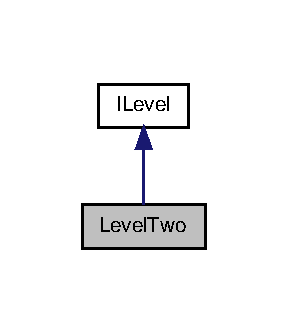
\includegraphics[width=138pt]{class_level_two__inherit__graph}
\end{center}
\end{figure}
\subsection*{Public Member Functions}
\begin{DoxyCompactItemize}
\item 
\hypertarget{class_level_two_ac57f1c4fa86d64e22a6d013af7afd886}{\hyperlink{class_level_two_ac57f1c4fa86d64e22a6d013af7afd886}{Level\-Two} (void)}\label{class_level_two_ac57f1c4fa86d64e22a6d013af7afd886}

\begin{DoxyCompactList}\small\item\em Default constructor. \end{DoxyCompactList}\item 
\hypertarget{class_level_two_aef76b8626bd780d32f3718f9a0000f68}{\hyperlink{class_level_two_aef76b8626bd780d32f3718f9a0000f68}{$\sim$\-Level\-Two} (void)}\label{class_level_two_aef76b8626bd780d32f3718f9a0000f68}

\begin{DoxyCompactList}\small\item\em Default destructor. \end{DoxyCompactList}\item 
int \hyperlink{class_level_two_a8c0c117bce3509249967c408b5e077a4}{get\-Height} (void)
\begin{DoxyCompactList}\small\item\em Get the height of the level. \end{DoxyCompactList}\item 
int \hyperlink{class_level_two_a8b5c8339077204363fc53e861710ca5c}{get\-Width} (void)
\begin{DoxyCompactList}\small\item\em Get the width of the level. \end{DoxyCompactList}\item 
virtual void \hyperlink{class_level_two_a71138ffe84dee9ed856a0328f3c72411}{load\-Level} (\hyperlink{class_player}{Player} $\ast$player)
\begin{DoxyCompactList}\small\item\em Load the level and the player according the tile map. \end{DoxyCompactList}\item 
virtual void \hyperlink{class_level_two_a6fbf138025c013260c7f572b41468a24}{draw\-Level} (sf\-::\-Render\-Window $\ast$screen)
\begin{DoxyCompactList}\small\item\em Draw all the elements of the level on the given screen. \end{DoxyCompactList}\item 
virtual std\-::vector\\*
$<$ sf\-::\-Sprite $\ast$ $>$ $\ast$ \hyperlink{class_level_two_a412f81d5b2b93ea6690635cc5ce02c8f}{get\-Blocks} (void)
\begin{DoxyCompactList}\small\item\em Get the blocks of the level. \end{DoxyCompactList}\item 
virtual sf\-::\-Sprite $\ast$ \hyperlink{class_level_two_a981cce04240b7d5bf4e5dc5b8a212319}{get\-End\-Sprite} (void)
\begin{DoxyCompactList}\small\item\em Get a pointer on the sprite of the end. \end{DoxyCompactList}\item 
virtual sf\-::\-Sprite $\ast$ \hyperlink{class_level_two_af9e5022cbec0fe1ec6171231374161dd}{get\-Cape\-Sprite} ()
\begin{DoxyCompactList}\small\item\em Get a pointer on the sprite of the cape. \end{DoxyCompactList}\item 
virtual sf\-::\-Sprite $\ast$ \hyperlink{class_level_two_ae382cc1e788e71eadcef2b5946ee204e}{get\-Shoes\-Sprite} ()
\begin{DoxyCompactList}\small\item\em Get a pointer on the sprite of the shoes. \end{DoxyCompactList}\item 
virtual void \hyperlink{class_level_two_a87ad50b6da9f82ecf602c789d354acae}{remove\-Element} (char target)
\begin{DoxyCompactList}\small\item\em Remove an element from the map. \end{DoxyCompactList}\item 
virtual \hyperlink{class_i_level}{I\-Level} $\ast$ \hyperlink{class_level_two_a4f0b0678a51169126fdd0e354ff4fa0e}{get\-Next} (void)
\begin{DoxyCompactList}\small\item\em Get the next level. \end{DoxyCompactList}\end{DoxyCompactItemize}
\subsection*{Private Attributes}
\begin{DoxyCompactItemize}
\item 
\hypertarget{class_level_two_a11ce0acdf2194208efcd706072a7ac6e}{std\-::vector$<$ std\-::string $>$ $\ast$ \hyperlink{class_level_two_a11ce0acdf2194208efcd706072a7ac6e}{m\-\_\-tile\-Map}}\label{class_level_two_a11ce0acdf2194208efcd706072a7ac6e}

\begin{DoxyCompactList}\small\item\em The tile map (i.\-e. the map of the level) \end{DoxyCompactList}\item 
\hypertarget{class_level_two_a05265df20ffedbd210a8bfdc7d20b350}{std\-::vector$<$ sf\-::\-Sprite $\ast$ $>$ $\ast$ \hyperlink{class_level_two_a05265df20ffedbd210a8bfdc7d20b350}{m\-\_\-blocks}}\label{class_level_two_a05265df20ffedbd210a8bfdc7d20b350}

\begin{DoxyCompactList}\small\item\em Contains all the elements of the level. \end{DoxyCompactList}\item 
\hypertarget{class_level_two_a6fda76adfb5f433935e26a25fa89cae5}{\hyperlink{class_i_block}{I\-Block} $\ast$ \hyperlink{class_level_two_a6fda76adfb5f433935e26a25fa89cae5}{m\-\_\-block}}\label{class_level_two_a6fda76adfb5f433935e26a25fa89cae5}

\begin{DoxyCompactList}\small\item\em Constructed block. \end{DoxyCompactList}\item 
\hypertarget{class_level_two_a67e50c63f7bd5805014d91c9acd44ef0}{sf\-::\-Texture $\ast$ \hyperlink{class_level_two_a67e50c63f7bd5805014d91c9acd44ef0}{m\-\_\-end\-Texture}}\label{class_level_two_a67e50c63f7bd5805014d91c9acd44ef0}

\begin{DoxyCompactList}\small\item\em Texture of the end sprite. \end{DoxyCompactList}\item 
\hypertarget{class_level_two_a8aed4e19d7cd859464602625d1f701ac}{sf\-::\-Sprite $\ast$ \hyperlink{class_level_two_a8aed4e19d7cd859464602625d1f701ac}{m\-\_\-end\-Sprite}}\label{class_level_two_a8aed4e19d7cd859464602625d1f701ac}

\begin{DoxyCompactList}\small\item\em Sprite of the end sprite. \end{DoxyCompactList}\item 
\hypertarget{class_level_two_a912c4e3e5e2e6fefbd2353778e110111}{\hyperlink{class_a_factory}{A\-Factory} $\ast$ \hyperlink{class_level_two_a912c4e3e5e2e6fefbd2353778e110111}{m\-\_\-factory}}\label{class_level_two_a912c4e3e5e2e6fefbd2353778e110111}

\begin{DoxyCompactList}\small\item\em The factory that will create the blocks. \end{DoxyCompactList}\item 
\hypertarget{class_level_two_a7aec6b6a58fbb0fb4836dd058937076a}{sf\-::\-Texture $\ast$ \hyperlink{class_level_two_a7aec6b6a58fbb0fb4836dd058937076a}{m\-\_\-cape\-Texture}}\label{class_level_two_a7aec6b6a58fbb0fb4836dd058937076a}

\begin{DoxyCompactList}\small\item\em \hyperlink{class_cape}{Cape} texture. \end{DoxyCompactList}\item 
\hypertarget{class_level_two_a6007c5a2be8b96f863a58c94683ad47b}{sf\-::\-Sprite $\ast$ \hyperlink{class_level_two_a6007c5a2be8b96f863a58c94683ad47b}{m\-\_\-cape\-Sprite}}\label{class_level_two_a6007c5a2be8b96f863a58c94683ad47b}

\begin{DoxyCompactList}\small\item\em \hyperlink{class_cape}{Cape} sprite. \end{DoxyCompactList}\item 
\hypertarget{class_level_two_adc6a65f9f141a466fff0e8343904e7af}{sf\-::\-Texture $\ast$ \hyperlink{class_level_two_adc6a65f9f141a466fff0e8343904e7af}{m\-\_\-shoes\-Texture}}\label{class_level_two_adc6a65f9f141a466fff0e8343904e7af}

\begin{DoxyCompactList}\small\item\em \hyperlink{class_shoes}{Shoes} texture. \end{DoxyCompactList}\item 
\hypertarget{class_level_two_af0eaf32e30de697697d1bace185fe29f}{sf\-::\-Sprite $\ast$ \hyperlink{class_level_two_af0eaf32e30de697697d1bace185fe29f}{m\-\_\-shoes\-Sprite}}\label{class_level_two_af0eaf32e30de697697d1bace185fe29f}

\begin{DoxyCompactList}\small\item\em \hyperlink{class_shoes}{Shoes} sprite. \end{DoxyCompactList}\item 
\hypertarget{class_level_two_a03014f87143fa101cd69dc0601916c20}{\hyperlink{class_i_level}{I\-Level} $\ast$ \hyperlink{class_level_two_a03014f87143fa101cd69dc0601916c20}{m\-\_\-next}}\label{class_level_two_a03014f87143fa101cd69dc0601916c20}

\begin{DoxyCompactList}\small\item\em Next level. \end{DoxyCompactList}\item 
\hypertarget{class_level_two_a094097697073aa1b33c71d70be269188}{bool \hyperlink{class_level_two_a094097697073aa1b33c71d70be269188}{m\-\_\-draw\-Cape}}\label{class_level_two_a094097697073aa1b33c71d70be269188}

\begin{DoxyCompactList}\small\item\em Boolean to know when the cape has to be draw or not. \end{DoxyCompactList}\item 
\hypertarget{class_level_two_abb41ddfe6e50c101fc35f8cf920b815d}{bool \hyperlink{class_level_two_abb41ddfe6e50c101fc35f8cf920b815d}{m\-\_\-draw\-Shoes}}\label{class_level_two_abb41ddfe6e50c101fc35f8cf920b815d}

\begin{DoxyCompactList}\small\item\em Boolean to know when the shoes has to be draw or not. \end{DoxyCompactList}\end{DoxyCompactItemize}


\subsection{Detailed Description}
Implements the second level of the game. 

\begin{DoxyAuthor}{Author}
Adrien Bodineau and Alexandre Gomes 
\end{DoxyAuthor}
\begin{DoxyVersion}{Version}
1.\-0 
\end{DoxyVersion}


\subsection{Member Function Documentation}
\hypertarget{class_level_two_a6fbf138025c013260c7f572b41468a24}{\index{Level\-Two@{Level\-Two}!draw\-Level@{draw\-Level}}
\index{draw\-Level@{draw\-Level}!LevelTwo@{Level\-Two}}
\subsubsection[{draw\-Level}]{\setlength{\rightskip}{0pt plus 5cm}void Level\-Two\-::draw\-Level (
\begin{DoxyParamCaption}
\item[{sf\-::\-Render\-Window $\ast$}]{screen}
\end{DoxyParamCaption}
)\hspace{0.3cm}{\ttfamily [virtual]}}}\label{class_level_two_a6fbf138025c013260c7f572b41468a24}


Draw all the elements of the level on the given screen. 


\begin{DoxyParams}{Parameters}
{\em screen} & The screen where the elements will be displayed \\
\hline
\end{DoxyParams}


Implements \hyperlink{class_i_level_a7e37723d1806e1c137c332fd4b28ba51}{I\-Level}.

\hypertarget{class_level_two_a412f81d5b2b93ea6690635cc5ce02c8f}{\index{Level\-Two@{Level\-Two}!get\-Blocks@{get\-Blocks}}
\index{get\-Blocks@{get\-Blocks}!LevelTwo@{Level\-Two}}
\subsubsection[{get\-Blocks}]{\setlength{\rightskip}{0pt plus 5cm}std\-::vector$<$ sf\-::\-Sprite $\ast$ $>$ $\ast$ Level\-Two\-::get\-Blocks (
\begin{DoxyParamCaption}
\item[{void}]{}
\end{DoxyParamCaption}
)\hspace{0.3cm}{\ttfamily [virtual]}}}\label{class_level_two_a412f81d5b2b93ea6690635cc5ce02c8f}


Get the blocks of the level. 

\begin{DoxyReturn}{Returns}
A vector with all the elements 
\end{DoxyReturn}


Implements \hyperlink{class_i_level_a9d3f0ff762fbb04038eac9de4531bc45}{I\-Level}.

\hypertarget{class_level_two_af9e5022cbec0fe1ec6171231374161dd}{\index{Level\-Two@{Level\-Two}!get\-Cape\-Sprite@{get\-Cape\-Sprite}}
\index{get\-Cape\-Sprite@{get\-Cape\-Sprite}!LevelTwo@{Level\-Two}}
\subsubsection[{get\-Cape\-Sprite}]{\setlength{\rightskip}{0pt plus 5cm}sf\-::\-Sprite $\ast$ Level\-Two\-::get\-Cape\-Sprite (
\begin{DoxyParamCaption}
\item[{void}]{}
\end{DoxyParamCaption}
)\hspace{0.3cm}{\ttfamily [virtual]}}}\label{class_level_two_af9e5022cbec0fe1ec6171231374161dd}


Get a pointer on the sprite of the cape. 

\begin{DoxyReturn}{Returns}
The pointer on the sprite of the cape 
\end{DoxyReturn}


Implements \hyperlink{class_i_level_a63d5e1443bff759199d0eb60b0f1eb1f}{I\-Level}.

\hypertarget{class_level_two_a981cce04240b7d5bf4e5dc5b8a212319}{\index{Level\-Two@{Level\-Two}!get\-End\-Sprite@{get\-End\-Sprite}}
\index{get\-End\-Sprite@{get\-End\-Sprite}!LevelTwo@{Level\-Two}}
\subsubsection[{get\-End\-Sprite}]{\setlength{\rightskip}{0pt plus 5cm}sf\-::\-Sprite $\ast$ Level\-Two\-::get\-End\-Sprite (
\begin{DoxyParamCaption}
\item[{void}]{}
\end{DoxyParamCaption}
)\hspace{0.3cm}{\ttfamily [virtual]}}}\label{class_level_two_a981cce04240b7d5bf4e5dc5b8a212319}


Get a pointer on the sprite of the end. 

\begin{DoxyReturn}{Returns}
The pointer on the sprite of the end 
\end{DoxyReturn}


Implements \hyperlink{class_i_level_a458fa2042948a69f5ec6951e77f9459e}{I\-Level}.

\hypertarget{class_level_two_a8c0c117bce3509249967c408b5e077a4}{\index{Level\-Two@{Level\-Two}!get\-Height@{get\-Height}}
\index{get\-Height@{get\-Height}!LevelTwo@{Level\-Two}}
\subsubsection[{get\-Height}]{\setlength{\rightskip}{0pt plus 5cm}int Level\-Two\-::get\-Height (
\begin{DoxyParamCaption}
\item[{void}]{}
\end{DoxyParamCaption}
)\hspace{0.3cm}{\ttfamily [virtual]}}}\label{class_level_two_a8c0c117bce3509249967c408b5e077a4}


Get the height of the level. 

\begin{DoxyReturn}{Returns}
The height of the level 
\end{DoxyReturn}


Implements \hyperlink{class_i_level_a192bb8106e09fb68794711b048ca748d}{I\-Level}.

\hypertarget{class_level_two_a4f0b0678a51169126fdd0e354ff4fa0e}{\index{Level\-Two@{Level\-Two}!get\-Next@{get\-Next}}
\index{get\-Next@{get\-Next}!LevelTwo@{Level\-Two}}
\subsubsection[{get\-Next}]{\setlength{\rightskip}{0pt plus 5cm}{\bf I\-Level} $\ast$ Level\-Two\-::get\-Next (
\begin{DoxyParamCaption}
\item[{void}]{}
\end{DoxyParamCaption}
)\hspace{0.3cm}{\ttfamily [virtual]}}}\label{class_level_two_a4f0b0678a51169126fdd0e354ff4fa0e}


Get the next level. 

\begin{DoxyReturn}{Returns}
Next level, N\-U\-L\-L if this is the last level 
\end{DoxyReturn}


Implements \hyperlink{class_i_level_a78b187489e43f061cbd990d9ae957178}{I\-Level}.

\hypertarget{class_level_two_ae382cc1e788e71eadcef2b5946ee204e}{\index{Level\-Two@{Level\-Two}!get\-Shoes\-Sprite@{get\-Shoes\-Sprite}}
\index{get\-Shoes\-Sprite@{get\-Shoes\-Sprite}!LevelTwo@{Level\-Two}}
\subsubsection[{get\-Shoes\-Sprite}]{\setlength{\rightskip}{0pt plus 5cm}sf\-::\-Sprite $\ast$ Level\-Two\-::get\-Shoes\-Sprite (
\begin{DoxyParamCaption}
\item[{void}]{}
\end{DoxyParamCaption}
)\hspace{0.3cm}{\ttfamily [virtual]}}}\label{class_level_two_ae382cc1e788e71eadcef2b5946ee204e}


Get a pointer on the sprite of the shoes. 

\begin{DoxyReturn}{Returns}
The pointer on the sprite of the shoes 
\end{DoxyReturn}


Implements \hyperlink{class_i_level_ac418e1773d0df3be6ddd40091f04689f}{I\-Level}.

\hypertarget{class_level_two_a8b5c8339077204363fc53e861710ca5c}{\index{Level\-Two@{Level\-Two}!get\-Width@{get\-Width}}
\index{get\-Width@{get\-Width}!LevelTwo@{Level\-Two}}
\subsubsection[{get\-Width}]{\setlength{\rightskip}{0pt plus 5cm}int Level\-Two\-::get\-Width (
\begin{DoxyParamCaption}
\item[{void}]{}
\end{DoxyParamCaption}
)\hspace{0.3cm}{\ttfamily [virtual]}}}\label{class_level_two_a8b5c8339077204363fc53e861710ca5c}


Get the width of the level. 

\begin{DoxyReturn}{Returns}
The width of the level 
\end{DoxyReturn}


Implements \hyperlink{class_i_level_a91daa2f5b760da916b348470cd5ed66e}{I\-Level}.

\hypertarget{class_level_two_a71138ffe84dee9ed856a0328f3c72411}{\index{Level\-Two@{Level\-Two}!load\-Level@{load\-Level}}
\index{load\-Level@{load\-Level}!LevelTwo@{Level\-Two}}
\subsubsection[{load\-Level}]{\setlength{\rightskip}{0pt plus 5cm}void Level\-Two\-::load\-Level (
\begin{DoxyParamCaption}
\item[{{\bf Player} $\ast$}]{player}
\end{DoxyParamCaption}
)\hspace{0.3cm}{\ttfamily [virtual]}}}\label{class_level_two_a71138ffe84dee9ed856a0328f3c72411}


Load the level and the player according the tile map. 


\begin{DoxyParams}{Parameters}
{\em player} & The pointer to the player, so the method can set his position \\
\hline
\end{DoxyParams}


Implements \hyperlink{class_i_level_ae5c21f7cc2cc8757ef50b767d4787138}{I\-Level}.

\hypertarget{class_level_two_a87ad50b6da9f82ecf602c789d354acae}{\index{Level\-Two@{Level\-Two}!remove\-Element@{remove\-Element}}
\index{remove\-Element@{remove\-Element}!LevelTwo@{Level\-Two}}
\subsubsection[{remove\-Element}]{\setlength{\rightskip}{0pt plus 5cm}void Level\-Two\-::remove\-Element (
\begin{DoxyParamCaption}
\item[{char}]{target}
\end{DoxyParamCaption}
)\hspace{0.3cm}{\ttfamily [virtual]}}}\label{class_level_two_a87ad50b6da9f82ecf602c789d354acae}


Remove an element from the map. 


\begin{DoxyParams}{Parameters}
{\em target} & Character representing the element to remove \\
\hline
\end{DoxyParams}


Implements \hyperlink{class_i_level_a185d4dd983c714a10a2bbdaebae202e6}{I\-Level}.


\hypertarget{class_menu}{\section{Menu Class Reference}
\label{class_menu}\index{Menu@{Menu}}
}


Game menu.  


\subsection*{Public Member Functions}
\begin{DoxyCompactItemize}
\item 
\hypertarget{class_menu_a73932d2ddab91e989102211f81c98c76}{virtual \hyperlink{class_menu_a73932d2ddab91e989102211f81c98c76}{$\sim$\-Menu} (void)}\label{class_menu_a73932d2ddab91e989102211f81c98c76}

\begin{DoxyCompactList}\small\item\em Default destructor. \end{DoxyCompactList}\item 
\hypertarget{class_menu_afbc7711526c62ad0d015bd8bf756b17e}{void \hyperlink{class_menu_afbc7711526c62ad0d015bd8bf756b17e}{action} (void)}\label{class_menu_afbc7711526c62ad0d015bd8bf756b17e}

\begin{DoxyCompactList}\small\item\em Method that implements the behavior of the menu. \end{DoxyCompactList}\end{DoxyCompactItemize}
\subsection*{Static Public Member Functions}
\begin{DoxyCompactItemize}
\item 
static \hyperlink{class_menu}{Menu} $\ast$ \hyperlink{class_menu_a93ed5d32c13c421c30bf6ef1291d7ec1}{get\-Instance} (void)
\begin{DoxyCompactList}\small\item\em Get menu instance. \end{DoxyCompactList}\end{DoxyCompactItemize}
\subsection*{Private Member Functions}
\begin{DoxyCompactItemize}
\item 
\hypertarget{class_menu_a0c1481a62f6b0bf63a506d2622f2244f}{\hyperlink{class_menu_a0c1481a62f6b0bf63a506d2622f2244f}{Menu} (void)}\label{class_menu_a0c1481a62f6b0bf63a506d2622f2244f}

\begin{DoxyCompactList}\small\item\em Private constructor. \end{DoxyCompactList}\end{DoxyCompactItemize}
\subsection*{Private Attributes}
\begin{DoxyCompactItemize}
\item 
\hypertarget{class_menu_a372778deb3a50ce92743ab3401c96324}{sf\-::\-Render\-Window $\ast$ \hyperlink{class_menu_a372778deb3a50ce92743ab3401c96324}{m\-\_\-screen}}\label{class_menu_a372778deb3a50ce92743ab3401c96324}

\begin{DoxyCompactList}\small\item\em Screen. \end{DoxyCompactList}\item 
\hypertarget{class_menu_a48dda7eda5fd21a5f82944302cfe49d4}{sf\-::\-Texture $\ast$ \hyperlink{class_menu_a48dda7eda5fd21a5f82944302cfe49d4}{m\-\_\-bg\-Texture}}\label{class_menu_a48dda7eda5fd21a5f82944302cfe49d4}

\begin{DoxyCompactList}\small\item\em Background texture. \end{DoxyCompactList}\item 
\hypertarget{class_menu_aa43a1797c926bd25f68dfb586f252486}{sf\-::\-Sprite $\ast$ \hyperlink{class_menu_aa43a1797c926bd25f68dfb586f252486}{m\-\_\-bg\-Sprite}}\label{class_menu_aa43a1797c926bd25f68dfb586f252486}

\begin{DoxyCompactList}\small\item\em Background sprite. \end{DoxyCompactList}\item 
\hypertarget{class_menu_a582d3e3b47317dcbf5125c1b902ef59d}{sf\-::\-Texture $\ast$ \hyperlink{class_menu_a582d3e3b47317dcbf5125c1b902ef59d}{m\-\_\-sax\-Texture}}\label{class_menu_a582d3e3b47317dcbf5125c1b902ef59d}

\begin{DoxyCompactList}\small\item\em Epic sax guy texture. \end{DoxyCompactList}\item 
\hypertarget{class_menu_a96ec3efb7af905a0c36d7919bc9b72c5}{sf\-::\-Texture $\ast$ \hyperlink{class_menu_a96ec3efb7af905a0c36d7919bc9b72c5}{m\-\_\-sax\-Dance\-Texture}}\label{class_menu_a96ec3efb7af905a0c36d7919bc9b72c5}

\begin{DoxyCompactList}\small\item\em Epic sax guy dance texture. \end{DoxyCompactList}\item 
\hypertarget{class_menu_ac907be23bf34e8cd7f05d5ea42d120e2}{sf\-::\-Texture $\ast$ \hyperlink{class_menu_ac907be23bf34e8cd7f05d5ea42d120e2}{m\-\_\-play\-Texture}}\label{class_menu_ac907be23bf34e8cd7f05d5ea42d120e2}

\begin{DoxyCompactList}\small\item\em Play button texture. \end{DoxyCompactList}\item 
\hypertarget{class_menu_ab0d75798058fe23875912f4b7f51f61b}{sf\-::\-Sprite $\ast$ \hyperlink{class_menu_ab0d75798058fe23875912f4b7f51f61b}{m\-\_\-play\-Sprite}}\label{class_menu_ab0d75798058fe23875912f4b7f51f61b}

\begin{DoxyCompactList}\small\item\em Play button sprite. \end{DoxyCompactList}\item 
\hypertarget{class_menu_a365d6ab154c7a1f15bcd1b36973127c4}{sf\-::\-Texture $\ast$ \hyperlink{class_menu_a365d6ab154c7a1f15bcd1b36973127c4}{m\-\_\-active\-Play\-Texture}}\label{class_menu_a365d6ab154c7a1f15bcd1b36973127c4}

\begin{DoxyCompactList}\small\item\em Active play button texture. \end{DoxyCompactList}\item 
\hypertarget{class_menu_a4abba58c2015794ec73539013b7c781d}{sf\-::\-Texture $\ast$ \hyperlink{class_menu_a4abba58c2015794ec73539013b7c781d}{m\-\_\-option\-Texture}}\label{class_menu_a4abba58c2015794ec73539013b7c781d}

\begin{DoxyCompactList}\small\item\em Option button texture. \end{DoxyCompactList}\item 
\hypertarget{class_menu_a2ec03c9cef485d448dda51c45380bb77}{sf\-::\-Sprite $\ast$ \hyperlink{class_menu_a2ec03c9cef485d448dda51c45380bb77}{m\-\_\-option\-Sprite}}\label{class_menu_a2ec03c9cef485d448dda51c45380bb77}

\begin{DoxyCompactList}\small\item\em Option button sprite. \end{DoxyCompactList}\item 
\hypertarget{class_menu_aec48becd56bbb565aaa14748b606e36e}{sf\-::\-Texture $\ast$ \hyperlink{class_menu_aec48becd56bbb565aaa14748b606e36e}{m\-\_\-active\-Option\-Texture}}\label{class_menu_aec48becd56bbb565aaa14748b606e36e}

\begin{DoxyCompactList}\small\item\em Active option button sprite. \end{DoxyCompactList}\item 
\hypertarget{class_menu_a42a8c6699db56e7dd57558c0824caa44}{sf\-::\-Music $\ast$ \hyperlink{class_menu_a42a8c6699db56e7dd57558c0824caa44}{m\-\_\-music}}\label{class_menu_a42a8c6699db56e7dd57558c0824caa44}

\begin{DoxyCompactList}\small\item\em Music of the game. \end{DoxyCompactList}\item 
\hypertarget{class_menu_a515800a21f18924b62fd3463ccf96f1b}{sf\-::\-Sound $\ast$ \hyperlink{class_menu_a515800a21f18924b62fd3463ccf96f1b}{m\-\_\-sound}}\label{class_menu_a515800a21f18924b62fd3463ccf96f1b}

\begin{DoxyCompactList}\small\item\em Sound of the buttons. \end{DoxyCompactList}\item 
\hypertarget{class_menu_a6516df7b5168d23891faf057571d9e1e}{sf\-::\-Sound\-Buffer $\ast$ \hyperlink{class_menu_a6516df7b5168d23891faf057571d9e1e}{m\-\_\-sound\-Buffer}}\label{class_menu_a6516df7b5168d23891faf057571d9e1e}

\begin{DoxyCompactList}\small\item\em Sound buffer of the buttons. \end{DoxyCompactList}\item 
\hypertarget{class_menu_add2ba5dc61b328bdc2c5559b929de940}{bool \hyperlink{class_menu_add2ba5dc61b328bdc2c5559b929de940}{m\-\_\-played}}\label{class_menu_add2ba5dc61b328bdc2c5559b929de940}

\begin{DoxyCompactList}\small\item\em Boolean to know when the buttons sound has to be played or not. \end{DoxyCompactList}\item 
\hypertarget{class_menu_accd3dfcde70f4e248ec11f9d1361003d}{bool \hyperlink{class_menu_accd3dfcde70f4e248ec11f9d1361003d}{m\-\_\-on\-Button}}\label{class_menu_accd3dfcde70f4e248ec11f9d1361003d}

\begin{DoxyCompactList}\small\item\em Boolean to know when the mouse is currently on the button. \end{DoxyCompactList}\item 
\hypertarget{class_menu_a468a4767b5ca00db10b36f4147f74879}{bool \hyperlink{class_menu_a468a4767b5ca00db10b36f4147f74879}{m\-\_\-saxguy}}\label{class_menu_a468a4767b5ca00db10b36f4147f74879}

\begin{DoxyCompactList}\small\item\em Boolean to know when the E\-P\-I\-C S\-A\-X G\-U\-Y mode is O\-N or O\-F\-F. \end{DoxyCompactList}\end{DoxyCompactItemize}
\subsection*{Static Private Attributes}
\begin{DoxyCompactItemize}
\item 
\hypertarget{class_menu_acbed43f19e618933f342ed95a5b12645}{static \hyperlink{class_menu}{Menu} $\ast$ \hyperlink{class_menu_acbed43f19e618933f342ed95a5b12645}{m\-\_\-menu}}\label{class_menu_acbed43f19e618933f342ed95a5b12645}

\begin{DoxyCompactList}\small\item\em Instance. \end{DoxyCompactList}\end{DoxyCompactItemize}


\subsection{Detailed Description}
Game menu. 

\begin{DoxyAuthor}{Author}
Adrien Bodineau and Alexandre Gomes 
\end{DoxyAuthor}
\begin{DoxyVersion}{Version}
1.\-0 
\end{DoxyVersion}


\subsection{Member Function Documentation}
\hypertarget{class_menu_a93ed5d32c13c421c30bf6ef1291d7ec1}{\index{Menu@{Menu}!get\-Instance@{get\-Instance}}
\index{get\-Instance@{get\-Instance}!Menu@{Menu}}
\subsubsection[{get\-Instance}]{\setlength{\rightskip}{0pt plus 5cm}static {\bf Menu} $\ast$ Menu\-::get\-Instance (
\begin{DoxyParamCaption}
\item[{void}]{}
\end{DoxyParamCaption}
)\hspace{0.3cm}{\ttfamily [inline]}, {\ttfamily [static]}}}\label{class_menu_a93ed5d32c13c421c30bf6ef1291d7ec1}


Get menu instance. 

\begin{DoxyReturn}{Returns}
\hyperlink{class_menu}{Menu} instance 
\end{DoxyReturn}

\hypertarget{class_player}{\section{Player Class Reference}
\label{class_player}\index{Player@{Player}}
}


\hyperlink{class_player}{Player} class.  




Inheritance diagram for Player\-:\nopagebreak
\begin{figure}[H]
\begin{center}
\leavevmode
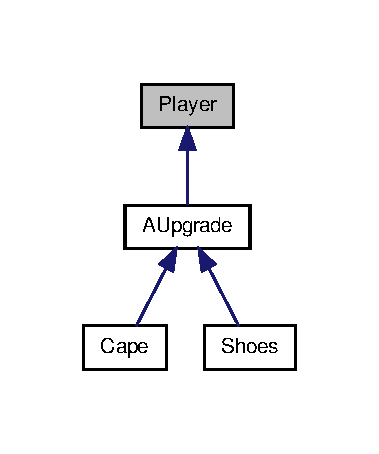
\includegraphics[width=182pt]{class_player__inherit__graph}
\end{center}
\end{figure}
\subsection*{Public Member Functions}
\begin{DoxyCompactItemize}
\item 
\hyperlink{class_player_a8e899b26bfec32ea70b2fbd983fa1ecc}{Player} (int x=0, int y=0)
\begin{DoxyCompactList}\small\item\em Default constructor. \end{DoxyCompactList}\item 
\hypertarget{class_player_a949762ad57300f070d83ec877ec6e907}{virtual \hyperlink{class_player_a949762ad57300f070d83ec877ec6e907}{$\sim$\-Player} (void)}\label{class_player_a949762ad57300f070d83ec877ec6e907}

\begin{DoxyCompactList}\small\item\em Default destructor. \end{DoxyCompactList}\item 
virtual void \hyperlink{class_player_aae6b7a837033bdd2338a200963f4309a}{set\-On\-Ground} (bool value)
\begin{DoxyCompactList}\small\item\em Set on\-Ground. \end{DoxyCompactList}\item 
\hypertarget{class_player_ade1f198046c99aa0a9a7b84b25e43621}{virtual void \hyperlink{class_player_ade1f198046c99aa0a9a7b84b25e43621}{go\-Right} (void)}\label{class_player_ade1f198046c99aa0a9a7b84b25e43621}

\begin{DoxyCompactList}\small\item\em Function to make the player go to the right. \end{DoxyCompactList}\item 
\hypertarget{class_player_ad5ec9b977afe277362f917883d18c2d2}{virtual void \hyperlink{class_player_ad5ec9b977afe277362f917883d18c2d2}{go\-Left} (void)}\label{class_player_ad5ec9b977afe277362f917883d18c2d2}

\begin{DoxyCompactList}\small\item\em Function to make the player go to the left. \end{DoxyCompactList}\item 
\hypertarget{class_player_a21d91a2eb70e1e4f9d8a60c11dcdd523}{virtual void \hyperlink{class_player_a21d91a2eb70e1e4f9d8a60c11dcdd523}{fall} (void)}\label{class_player_a21d91a2eb70e1e4f9d8a60c11dcdd523}

\begin{DoxyCompactList}\small\item\em Function to make the player fall. \end{DoxyCompactList}\item 
virtual void \hyperlink{class_player_a2dea085dd04cc2d2c0a73950b8f6383b}{controls} (char collision\-R, char collision\-L, char collision\-T, char collision\-G)
\begin{DoxyCompactList}\small\item\em Indicate what the player have to do according to the collisions and the press buttons. \end{DoxyCompactList}\item 
\hypertarget{class_player_a0ccf6995405ca7f8efd159117eb332c6}{virtual void \hyperlink{class_player_a0ccf6995405ca7f8efd159117eb332c6}{jump} (void)}\label{class_player_a0ccf6995405ca7f8efd159117eb332c6}

\begin{DoxyCompactList}\small\item\em Set up the jump. \end{DoxyCompactList}\item 
virtual void \hyperlink{class_player_af0cbf262b74bd173c708e32a1df22c4b}{jump\-Animation} (char collision\-R, char collision\-L, char collision\-T, char collision\-G)
\begin{DoxyCompactList}\small\item\em Make the player jump. \end{DoxyCompactList}\item 
virtual void \hyperlink{class_player_ae71f2d49d8ae2482210981745e699318}{set\-Jumping} (bool value)
\begin{DoxyCompactList}\small\item\em Set the jumping value. \end{DoxyCompactList}\item 
virtual void \hyperlink{class_player_afe708570bc166a91649478dd22108e7a}{set\-Speed} (int speed)
\begin{DoxyCompactList}\small\item\em Set the speed value. \end{DoxyCompactList}\item 
virtual void \hyperlink{class_player_ada5c4c79a954c38fb5d329666d78a379}{set\-Jump\-Speed} (int jump\-Speed)
\begin{DoxyCompactList}\small\item\em Set the jumping speed value. \end{DoxyCompactList}\item 
virtual void \hyperlink{class_player_ad5a29d64aae25aaa440283866b74509b}{set\-Jump\-Height} (int jump\-Height)
\begin{DoxyCompactList}\small\item\em Set the jumping height value. \end{DoxyCompactList}\item 
virtual sf\-::\-Int\-Rect $\ast$ \hyperlink{class_player_a1967129b1085527e58d605bc657f80ff}{get\-Rect} (void)
\begin{DoxyCompactList}\small\item\em Get the rect of the player. \end{DoxyCompactList}\item 
virtual bool \hyperlink{class_player_a803903a8eae317b46d3ecd22babb231f}{get\-Jumping} (void)
\begin{DoxyCompactList}\small\item\em Get the jumping value. \end{DoxyCompactList}\item 
virtual int \hyperlink{class_player_a5755be9818f6f911d9494e4948d8c483}{get\-Speed} ()
\begin{DoxyCompactList}\small\item\em Get the speed value. \end{DoxyCompactList}\item 
virtual int \hyperlink{class_player_a95676c9d2da2c6e778aa8558c5e5fa80}{get\-Jump\-Speed} ()
\begin{DoxyCompactList}\small\item\em Get the jumping speed value. \end{DoxyCompactList}\item 
virtual int \hyperlink{class_player_a4df8845cc35f7ef2d8aefbeffb141aed}{get\-Jump\-Height} ()
\begin{DoxyCompactList}\small\item\em Get the jumping height value. \end{DoxyCompactList}\item 
virtual sf\-::\-Sprite $\ast$ \hyperlink{class_player_adbce087693a5623afac017735d67a39d}{get\-Sprite} (void)
\begin{DoxyCompactList}\small\item\em Get the sprite of the player. \end{DoxyCompactList}\item 
virtual bool \hyperlink{class_player_a79eac778dc97f959fd3f82e7807b54af}{get\-On\-Ground} (void)
\begin{DoxyCompactList}\small\item\em Get the boolean on\-Ground. \end{DoxyCompactList}\item 
virtual int \hyperlink{class_player_af80fb70e7b808f24192b49ca0f5656f0}{get\-Position\-X} (int inc=0)
\begin{DoxyCompactList}\small\item\em Get the position x. \end{DoxyCompactList}\item 
virtual int \hyperlink{class_player_a04dfb18ee251361671bad38cf0d42a4a}{get\-Position\-Y} (int inc=0)
\begin{DoxyCompactList}\small\item\em Get the position y. \end{DoxyCompactList}\item 
virtual int \hyperlink{class_player_a758ed6885202cac4e51e9022c1371afa}{get\-Width} (int inc=0)
\begin{DoxyCompactList}\small\item\em Get the player's width. \end{DoxyCompactList}\item 
virtual int \hyperlink{class_player_af215d8b616713cbbb1ab6207d26fffde}{get\-Height} (int inc=0)
\begin{DoxyCompactList}\small\item\em Get the player's height. \end{DoxyCompactList}\item 
virtual sf\-::\-Texture $\ast$ \hyperlink{class_player_aa0452c12db96c7d4dd9fd3c93ad2bbb1}{get\-Texture} ()
\begin{DoxyCompactList}\small\item\em Get the player's texture. \end{DoxyCompactList}\item 
virtual sf\-::\-Texture $\ast$ \hyperlink{class_player_a5bdf81d3fb9358acae70ac51e818fa84}{get\-Run\-Texture1} ()
\begin{DoxyCompactList}\small\item\em Get the player's run texture 1. \end{DoxyCompactList}\item 
virtual sf\-::\-Texture $\ast$ \hyperlink{class_player_afd441d4a8f47d23eeb91b362d0da3533}{get\-Run\-Texture2} ()
\begin{DoxyCompactList}\small\item\em Get the player's run texture 2. \end{DoxyCompactList}\item 
virtual sf\-::\-Texture $\ast$ \hyperlink{class_player_aea67670a94415f077ac15f4dd85ea6e6}{get\-Run\-Texture3} ()
\begin{DoxyCompactList}\small\item\em Get the player's run texture 3. \end{DoxyCompactList}\item 
virtual sf\-::\-Texture $\ast$ \hyperlink{class_player_a8d9efc602e8feb4dbb64535ed4e110bd}{get\-Run\-Texture4} ()
\begin{DoxyCompactList}\small\item\em Get the player's run texture 4. \end{DoxyCompactList}\item 
virtual sf\-::\-Texture $\ast$ \hyperlink{class_player_a9933563897756d9066b0a700978d91ec}{get\-Run\-Texture5} ()
\begin{DoxyCompactList}\small\item\em Get the player's run texture 5. \end{DoxyCompactList}\item 
virtual sf\-::\-Texture $\ast$ \hyperlink{class_player_a4869df8bb0be21e6c6f84fb708d01fa5}{get\-Run\-Texture6} ()
\begin{DoxyCompactList}\small\item\em Get the player's run texture 6. \end{DoxyCompactList}\item 
virtual sf\-::\-Sound $\ast$ \hyperlink{class_player_a0056edff24f3cc0110425386bd6fcdb2}{get\-Jump\-Sound} ()
\begin{DoxyCompactList}\small\item\em Get the jump sound. \end{DoxyCompactList}\item 
virtual sf\-::\-Sound\-Buffer $\ast$ \hyperlink{class_player_ae34ef062d527edbcaf6070544bea312e}{get\-Jump\-Sound\-Buffer} ()
\begin{DoxyCompactList}\small\item\em Get the jump sound buffer. \end{DoxyCompactList}\item 
virtual int \hyperlink{class_player_a5ce5ed6ed57130731accbd8980a65695}{get\-Jump} ()
\begin{DoxyCompactList}\small\item\em Get the value of jump. \end{DoxyCompactList}\item 
virtual double \hyperlink{class_player_a3fa494de13eaaad0280d6d2017ae85a9}{get\-Current\-Frame} ()
\begin{DoxyCompactList}\small\item\em Get the player's current frame. \end{DoxyCompactList}\end{DoxyCompactItemize}
\subsection*{Protected Attributes}
\begin{DoxyCompactItemize}
\item 
\hypertarget{class_player_aba34d2ce20f5ab84c38c287a7e16e497}{sf\-::\-Texture $\ast$ \hyperlink{class_player_aba34d2ce20f5ab84c38c287a7e16e497}{m\-\_\-texture}}\label{class_player_aba34d2ce20f5ab84c38c287a7e16e497}

\begin{DoxyCompactList}\small\item\em \hyperlink{class_player}{Player}'s texture. \end{DoxyCompactList}\item 
\hypertarget{class_player_ab1123072990bf0605849f6e4a66550da}{sf\-::\-Texture $\ast$ \hyperlink{class_player_ab1123072990bf0605849f6e4a66550da}{m\-\_\-run\-Texture1}}\label{class_player_ab1123072990bf0605849f6e4a66550da}

\begin{DoxyCompactList}\small\item\em \hyperlink{class_player}{Player}'s run texture 1. \end{DoxyCompactList}\item 
\hypertarget{class_player_af470f29584a4b4a994cdbcbd8572b1f6}{sf\-::\-Texture $\ast$ \hyperlink{class_player_af470f29584a4b4a994cdbcbd8572b1f6}{m\-\_\-run\-Texture2}}\label{class_player_af470f29584a4b4a994cdbcbd8572b1f6}

\begin{DoxyCompactList}\small\item\em \hyperlink{class_player}{Player}'s run texture 2. \end{DoxyCompactList}\item 
\hypertarget{class_player_abd4d5c0efb97dd1342969bfb5e935c84}{sf\-::\-Texture $\ast$ \hyperlink{class_player_abd4d5c0efb97dd1342969bfb5e935c84}{m\-\_\-run\-Texture3}}\label{class_player_abd4d5c0efb97dd1342969bfb5e935c84}

\begin{DoxyCompactList}\small\item\em \hyperlink{class_player}{Player}'s run texture 3. \end{DoxyCompactList}\item 
\hypertarget{class_player_a556553a62c2db12bb1b57721e59a58d7}{sf\-::\-Texture $\ast$ \hyperlink{class_player_a556553a62c2db12bb1b57721e59a58d7}{m\-\_\-run\-Texture4}}\label{class_player_a556553a62c2db12bb1b57721e59a58d7}

\begin{DoxyCompactList}\small\item\em \hyperlink{class_player}{Player}'s run texture 4. \end{DoxyCompactList}\item 
\hypertarget{class_player_a2f8d3aa38eff7616e9945928c24327fb}{sf\-::\-Texture $\ast$ \hyperlink{class_player_a2f8d3aa38eff7616e9945928c24327fb}{m\-\_\-run\-Texture5}}\label{class_player_a2f8d3aa38eff7616e9945928c24327fb}

\begin{DoxyCompactList}\small\item\em \hyperlink{class_player}{Player}'s run texture 5. \end{DoxyCompactList}\item 
\hypertarget{class_player_aa6c3d3e02f5fd134673048aa45f48885}{sf\-::\-Texture $\ast$ \hyperlink{class_player_aa6c3d3e02f5fd134673048aa45f48885}{m\-\_\-run\-Texture6}}\label{class_player_aa6c3d3e02f5fd134673048aa45f48885}

\begin{DoxyCompactList}\small\item\em \hyperlink{class_player}{Player}'s run texture 6. \end{DoxyCompactList}\item 
\hypertarget{class_player_adadc7846bd20ea1e375340e99173a28f}{sf\-::\-Texture $\ast$ \hyperlink{class_player_adadc7846bd20ea1e375340e99173a28f}{m\-\_\-anim\-Tab} \mbox{[}6\mbox{]}}\label{class_player_adadc7846bd20ea1e375340e99173a28f}

\begin{DoxyCompactList}\small\item\em Array of the run textures. \end{DoxyCompactList}\item 
\hypertarget{class_player_a83c449829335b613129c47e9f3293b9c}{sf\-::\-Texture $\ast$ \hyperlink{class_player_a83c449829335b613129c47e9f3293b9c}{m\-\_\-jump\-Texture}}\label{class_player_a83c449829335b613129c47e9f3293b9c}

\begin{DoxyCompactList}\small\item\em \hyperlink{class_player}{Player}'s jump texture. \end{DoxyCompactList}\item 
\hypertarget{class_player_a2fe5d004be97d41e6c15979b449ab65c}{sf\-::\-Texture $\ast$ \hyperlink{class_player_a2fe5d004be97d41e6c15979b449ab65c}{m\-\_\-fall\-Texture}}\label{class_player_a2fe5d004be97d41e6c15979b449ab65c}

\begin{DoxyCompactList}\small\item\em \hyperlink{class_player}{Player}'s fall texture. \end{DoxyCompactList}\item 
\hypertarget{class_player_a06b952ac7dc29ec9ca7374c41ececb36}{sf\-::\-Sprite $\ast$ \hyperlink{class_player_a06b952ac7dc29ec9ca7374c41ececb36}{m\-\_\-sprite}}\label{class_player_a06b952ac7dc29ec9ca7374c41ececb36}

\begin{DoxyCompactList}\small\item\em \hyperlink{class_player}{Player}'s sprite. \end{DoxyCompactList}\item 
\hypertarget{class_player_a1586ec20fe0ab3172bbe4b7fed22b028}{sf\-::\-Sound $\ast$ \hyperlink{class_player_a1586ec20fe0ab3172bbe4b7fed22b028}{m\-\_\-jump\-Sound}}\label{class_player_a1586ec20fe0ab3172bbe4b7fed22b028}

\begin{DoxyCompactList}\small\item\em Jump sound. \end{DoxyCompactList}\item 
\hypertarget{class_player_ada9922e4960f83ff5e7135aeccd07848}{sf\-::\-Sound\-Buffer $\ast$ \hyperlink{class_player_ada9922e4960f83ff5e7135aeccd07848}{m\-\_\-jump\-Sound\-Buffer}}\label{class_player_ada9922e4960f83ff5e7135aeccd07848}

\begin{DoxyCompactList}\small\item\em Jump sound buffer. \end{DoxyCompactList}\item 
\hypertarget{class_player_a0ed905d7ce35dc1bb142861d97955e2e}{sf\-::\-Int\-Rect $\ast$ \hyperlink{class_player_a0ed905d7ce35dc1bb142861d97955e2e}{m\-\_\-rect}}\label{class_player_a0ed905d7ce35dc1bb142861d97955e2e}

\begin{DoxyCompactList}\small\item\em \hyperlink{class_player}{Player}'s rect. \end{DoxyCompactList}\item 
\hypertarget{class_player_a038a574bcbe535460f024c28b5348191}{int \hyperlink{class_player_a038a574bcbe535460f024c28b5348191}{m\-\_\-dx}}\label{class_player_a038a574bcbe535460f024c28b5348191}

\begin{DoxyCompactList}\small\item\em Position x. \end{DoxyCompactList}\item 
\hypertarget{class_player_a699a186e9a37c898f938c21e6a086821}{int \hyperlink{class_player_a699a186e9a37c898f938c21e6a086821}{m\-\_\-dy}}\label{class_player_a699a186e9a37c898f938c21e6a086821}

\begin{DoxyCompactList}\small\item\em Position y. \end{DoxyCompactList}\item 
\hypertarget{class_player_a4f3be31c677f7c86cd838381b418d440}{bool \hyperlink{class_player_a4f3be31c677f7c86cd838381b418d440}{m\-\_\-on\-Ground}}\label{class_player_a4f3be31c677f7c86cd838381b418d440}

\begin{DoxyCompactList}\small\item\em Boolean to know if the player is on the ground. \end{DoxyCompactList}\item 
\hypertarget{class_player_a38b5de5aa041c1766c572c046feb0f08}{bool \hyperlink{class_player_a38b5de5aa041c1766c572c046feb0f08}{m\-\_\-jumping}}\label{class_player_a38b5de5aa041c1766c572c046feb0f08}

\begin{DoxyCompactList}\small\item\em Boolean to know if the player is jumping. \end{DoxyCompactList}\item 
\hypertarget{class_player_a87196b22a09b01735cfc6e0eb3a4ad62}{int \hyperlink{class_player_a87196b22a09b01735cfc6e0eb3a4ad62}{m\-\_\-jump}}\label{class_player_a87196b22a09b01735cfc6e0eb3a4ad62}

\begin{DoxyCompactList}\small\item\em Value of the jump. \end{DoxyCompactList}\item 
\hypertarget{class_player_aa1f75eb3abbb09f12c21f071a2b13b95}{double \hyperlink{class_player_aa1f75eb3abbb09f12c21f071a2b13b95}{m\-\_\-current\-Frame}}\label{class_player_aa1f75eb3abbb09f12c21f071a2b13b95}

\begin{DoxyCompactList}\small\item\em Value of the current frame. \end{DoxyCompactList}\item 
\hypertarget{class_player_a3b350d804ed50bf5acdc5069a98e7a8a}{int \hyperlink{class_player_a3b350d804ed50bf5acdc5069a98e7a8a}{m\-\_\-speed}}\label{class_player_a3b350d804ed50bf5acdc5069a98e7a8a}

\begin{DoxyCompactList}\small\item\em \hyperlink{class_player}{Player}'s speed. \end{DoxyCompactList}\item 
\hypertarget{class_player_ac89446b6b822013a15388a5536bc2a36}{int \hyperlink{class_player_ac89446b6b822013a15388a5536bc2a36}{m\-\_\-jump\-Speed}}\label{class_player_ac89446b6b822013a15388a5536bc2a36}

\begin{DoxyCompactList}\small\item\em Jump speed. \end{DoxyCompactList}\item 
\hypertarget{class_player_a0d84b6cf8840e0c226943d4962c99eda}{int \hyperlink{class_player_a0d84b6cf8840e0c226943d4962c99eda}{m\-\_\-jump\-Height}}\label{class_player_a0d84b6cf8840e0c226943d4962c99eda}

\begin{DoxyCompactList}\small\item\em Jump height. \end{DoxyCompactList}\end{DoxyCompactItemize}


\subsection{Detailed Description}
\hyperlink{class_player}{Player} class. 

\begin{DoxyAuthor}{Author}
Adrien Bodineau and Alexandre Gomes 
\end{DoxyAuthor}
\begin{DoxyVersion}{Version}
1.\-0 
\end{DoxyVersion}


\subsection{Constructor \& Destructor Documentation}
\hypertarget{class_player_a8e899b26bfec32ea70b2fbd983fa1ecc}{\index{Player@{Player}!Player@{Player}}
\index{Player@{Player}!Player@{Player}}
\subsubsection[{Player}]{\setlength{\rightskip}{0pt plus 5cm}Player\-::\-Player (
\begin{DoxyParamCaption}
\item[{int}]{x = {\ttfamily 0}, }
\item[{int}]{y = {\ttfamily 0}}
\end{DoxyParamCaption}
)}}\label{class_player_a8e899b26bfec32ea70b2fbd983fa1ecc}


Default constructor. 


\begin{DoxyParams}{Parameters}
{\em x} & Position x \\
\hline
{\em y} & Position y \\
\hline
\end{DoxyParams}


\subsection{Member Function Documentation}
\hypertarget{class_player_a2dea085dd04cc2d2c0a73950b8f6383b}{\index{Player@{Player}!controls@{controls}}
\index{controls@{controls}!Player@{Player}}
\subsubsection[{controls}]{\setlength{\rightskip}{0pt plus 5cm}void Player\-::controls (
\begin{DoxyParamCaption}
\item[{char}]{collision\-R, }
\item[{char}]{collision\-L, }
\item[{char}]{collision\-T, }
\item[{char}]{collision\-G}
\end{DoxyParamCaption}
)\hspace{0.3cm}{\ttfamily [virtual]}}}\label{class_player_a2dea085dd04cc2d2c0a73950b8f6383b}


Indicate what the player have to do according to the collisions and the press buttons. 


\begin{DoxyParams}{Parameters}
{\em collision\-R} & Character to indicate the right collision \\
\hline
{\em collision\-L} & Character to indicate the left collision \\
\hline
{\em collision\-T} & Character to indicate the top collision \\
\hline
{\em collision\-G} & Character to indicate the ground collision \\
\hline
\end{DoxyParams}
\hypertarget{class_player_a3fa494de13eaaad0280d6d2017ae85a9}{\index{Player@{Player}!get\-Current\-Frame@{get\-Current\-Frame}}
\index{get\-Current\-Frame@{get\-Current\-Frame}!Player@{Player}}
\subsubsection[{get\-Current\-Frame}]{\setlength{\rightskip}{0pt plus 5cm}double Player\-::get\-Current\-Frame (
\begin{DoxyParamCaption}
{}
\end{DoxyParamCaption}
)\hspace{0.3cm}{\ttfamily [virtual]}}}\label{class_player_a3fa494de13eaaad0280d6d2017ae85a9}


Get the player's current frame. 

\begin{DoxyReturn}{Returns}
\hyperlink{class_player}{Player}'s current frame 
\end{DoxyReturn}
\hypertarget{class_player_af215d8b616713cbbb1ab6207d26fffde}{\index{Player@{Player}!get\-Height@{get\-Height}}
\index{get\-Height@{get\-Height}!Player@{Player}}
\subsubsection[{get\-Height}]{\setlength{\rightskip}{0pt plus 5cm}int Player\-::get\-Height (
\begin{DoxyParamCaption}
\item[{int}]{inc = {\ttfamily 0}}
\end{DoxyParamCaption}
)\hspace{0.3cm}{\ttfamily [virtual]}}}\label{class_player_af215d8b616713cbbb1ab6207d26fffde}


Get the player's height. 

\begin{DoxyReturn}{Returns}
\hyperlink{class_player}{Player}'s height 
\end{DoxyReturn}
\hypertarget{class_player_a5ce5ed6ed57130731accbd8980a65695}{\index{Player@{Player}!get\-Jump@{get\-Jump}}
\index{get\-Jump@{get\-Jump}!Player@{Player}}
\subsubsection[{get\-Jump}]{\setlength{\rightskip}{0pt plus 5cm}int Player\-::get\-Jump (
\begin{DoxyParamCaption}
{}
\end{DoxyParamCaption}
)\hspace{0.3cm}{\ttfamily [virtual]}}}\label{class_player_a5ce5ed6ed57130731accbd8980a65695}


Get the value of jump. 

\begin{DoxyReturn}{Returns}
Jump value 
\end{DoxyReturn}
\hypertarget{class_player_a4df8845cc35f7ef2d8aefbeffb141aed}{\index{Player@{Player}!get\-Jump\-Height@{get\-Jump\-Height}}
\index{get\-Jump\-Height@{get\-Jump\-Height}!Player@{Player}}
\subsubsection[{get\-Jump\-Height}]{\setlength{\rightskip}{0pt plus 5cm}int Player\-::get\-Jump\-Height (
\begin{DoxyParamCaption}
{}
\end{DoxyParamCaption}
)\hspace{0.3cm}{\ttfamily [virtual]}}}\label{class_player_a4df8845cc35f7ef2d8aefbeffb141aed}


Get the jumping height value. 

\begin{DoxyReturn}{Returns}
Jumping height value 
\end{DoxyReturn}


Reimplemented in \hyperlink{class_cape_ac2a629b66fc5b2678ebf294523b53799}{Cape}, and \hyperlink{class_shoes_a25361fa44b1f513548fe717b6befd53d}{Shoes}.

\hypertarget{class_player_a803903a8eae317b46d3ecd22babb231f}{\index{Player@{Player}!get\-Jumping@{get\-Jumping}}
\index{get\-Jumping@{get\-Jumping}!Player@{Player}}
\subsubsection[{get\-Jumping}]{\setlength{\rightskip}{0pt plus 5cm}bool Player\-::get\-Jumping (
\begin{DoxyParamCaption}
\item[{void}]{}
\end{DoxyParamCaption}
)\hspace{0.3cm}{\ttfamily [virtual]}}}\label{class_player_a803903a8eae317b46d3ecd22babb231f}


Get the jumping value. 

\begin{DoxyReturn}{Returns}
Jumping value 
\end{DoxyReturn}
\hypertarget{class_player_a0056edff24f3cc0110425386bd6fcdb2}{\index{Player@{Player}!get\-Jump\-Sound@{get\-Jump\-Sound}}
\index{get\-Jump\-Sound@{get\-Jump\-Sound}!Player@{Player}}
\subsubsection[{get\-Jump\-Sound}]{\setlength{\rightskip}{0pt plus 5cm}sf\-::\-Sound $\ast$ Player\-::get\-Jump\-Sound (
\begin{DoxyParamCaption}
{}
\end{DoxyParamCaption}
)\hspace{0.3cm}{\ttfamily [virtual]}}}\label{class_player_a0056edff24f3cc0110425386bd6fcdb2}


Get the jump sound. 

\begin{DoxyReturn}{Returns}
Jump sound 
\end{DoxyReturn}
\hypertarget{class_player_ae34ef062d527edbcaf6070544bea312e}{\index{Player@{Player}!get\-Jump\-Sound\-Buffer@{get\-Jump\-Sound\-Buffer}}
\index{get\-Jump\-Sound\-Buffer@{get\-Jump\-Sound\-Buffer}!Player@{Player}}
\subsubsection[{get\-Jump\-Sound\-Buffer}]{\setlength{\rightskip}{0pt plus 5cm}sf\-::\-Sound\-Buffer $\ast$ Player\-::get\-Jump\-Sound\-Buffer (
\begin{DoxyParamCaption}
{}
\end{DoxyParamCaption}
)\hspace{0.3cm}{\ttfamily [virtual]}}}\label{class_player_ae34ef062d527edbcaf6070544bea312e}


Get the jump sound buffer. 

\begin{DoxyReturn}{Returns}
Jump sound buffer 
\end{DoxyReturn}
\hypertarget{class_player_a95676c9d2da2c6e778aa8558c5e5fa80}{\index{Player@{Player}!get\-Jump\-Speed@{get\-Jump\-Speed}}
\index{get\-Jump\-Speed@{get\-Jump\-Speed}!Player@{Player}}
\subsubsection[{get\-Jump\-Speed}]{\setlength{\rightskip}{0pt plus 5cm}int Player\-::get\-Jump\-Speed (
\begin{DoxyParamCaption}
{}
\end{DoxyParamCaption}
)\hspace{0.3cm}{\ttfamily [virtual]}}}\label{class_player_a95676c9d2da2c6e778aa8558c5e5fa80}


Get the jumping speed value. 

\begin{DoxyReturn}{Returns}
Jump speed value 
\end{DoxyReturn}


Reimplemented in \hyperlink{class_cape_a2b563a9b4bd336530dfe01585123a087}{Cape}, and \hyperlink{class_shoes_a61b25a380629e60aa9996dc05a8db0df}{Shoes}.

\hypertarget{class_player_a79eac778dc97f959fd3f82e7807b54af}{\index{Player@{Player}!get\-On\-Ground@{get\-On\-Ground}}
\index{get\-On\-Ground@{get\-On\-Ground}!Player@{Player}}
\subsubsection[{get\-On\-Ground}]{\setlength{\rightskip}{0pt plus 5cm}bool Player\-::get\-On\-Ground (
\begin{DoxyParamCaption}
\item[{void}]{}
\end{DoxyParamCaption}
)\hspace{0.3cm}{\ttfamily [virtual]}}}\label{class_player_a79eac778dc97f959fd3f82e7807b54af}


Get the boolean on\-Ground. 

\begin{DoxyReturn}{Returns}
Value of on\-Ground 
\end{DoxyReturn}
\hypertarget{class_player_af80fb70e7b808f24192b49ca0f5656f0}{\index{Player@{Player}!get\-Position\-X@{get\-Position\-X}}
\index{get\-Position\-X@{get\-Position\-X}!Player@{Player}}
\subsubsection[{get\-Position\-X}]{\setlength{\rightskip}{0pt plus 5cm}int Player\-::get\-Position\-X (
\begin{DoxyParamCaption}
\item[{int}]{inc = {\ttfamily 0}}
\end{DoxyParamCaption}
)\hspace{0.3cm}{\ttfamily [virtual]}}}\label{class_player_af80fb70e7b808f24192b49ca0f5656f0}


Get the position x. 


\begin{DoxyParams}{Parameters}
{\em inc} & Get the position x+inc \\
\hline
\end{DoxyParams}
\begin{DoxyReturn}{Returns}
Position x 
\end{DoxyReturn}
\hypertarget{class_player_a04dfb18ee251361671bad38cf0d42a4a}{\index{Player@{Player}!get\-Position\-Y@{get\-Position\-Y}}
\index{get\-Position\-Y@{get\-Position\-Y}!Player@{Player}}
\subsubsection[{get\-Position\-Y}]{\setlength{\rightskip}{0pt plus 5cm}int Player\-::get\-Position\-Y (
\begin{DoxyParamCaption}
\item[{int}]{inc = {\ttfamily 0}}
\end{DoxyParamCaption}
)\hspace{0.3cm}{\ttfamily [virtual]}}}\label{class_player_a04dfb18ee251361671bad38cf0d42a4a}


Get the position y. 


\begin{DoxyParams}{Parameters}
{\em inc} & Get the position y+inc \\
\hline
\end{DoxyParams}
\begin{DoxyReturn}{Returns}
Position y 
\end{DoxyReturn}
\hypertarget{class_player_a1967129b1085527e58d605bc657f80ff}{\index{Player@{Player}!get\-Rect@{get\-Rect}}
\index{get\-Rect@{get\-Rect}!Player@{Player}}
\subsubsection[{get\-Rect}]{\setlength{\rightskip}{0pt plus 5cm}sf\-::\-Int\-Rect $\ast$ Player\-::get\-Rect (
\begin{DoxyParamCaption}
\item[{void}]{}
\end{DoxyParamCaption}
)\hspace{0.3cm}{\ttfamily [virtual]}}}\label{class_player_a1967129b1085527e58d605bc657f80ff}


Get the rect of the player. 

\begin{DoxyReturn}{Returns}
\hyperlink{class_player}{Player}'s rect 
\end{DoxyReturn}
\hypertarget{class_player_a5bdf81d3fb9358acae70ac51e818fa84}{\index{Player@{Player}!get\-Run\-Texture1@{get\-Run\-Texture1}}
\index{get\-Run\-Texture1@{get\-Run\-Texture1}!Player@{Player}}
\subsubsection[{get\-Run\-Texture1}]{\setlength{\rightskip}{0pt plus 5cm}sf\-::\-Texture $\ast$ Player\-::get\-Run\-Texture1 (
\begin{DoxyParamCaption}
{}
\end{DoxyParamCaption}
)\hspace{0.3cm}{\ttfamily [virtual]}}}\label{class_player_a5bdf81d3fb9358acae70ac51e818fa84}


Get the player's run texture 1. 

\begin{DoxyReturn}{Returns}
\hyperlink{class_player}{Player}'s run texture 1 
\end{DoxyReturn}
\hypertarget{class_player_afd441d4a8f47d23eeb91b362d0da3533}{\index{Player@{Player}!get\-Run\-Texture2@{get\-Run\-Texture2}}
\index{get\-Run\-Texture2@{get\-Run\-Texture2}!Player@{Player}}
\subsubsection[{get\-Run\-Texture2}]{\setlength{\rightskip}{0pt plus 5cm}sf\-::\-Texture $\ast$ Player\-::get\-Run\-Texture2 (
\begin{DoxyParamCaption}
{}
\end{DoxyParamCaption}
)\hspace{0.3cm}{\ttfamily [virtual]}}}\label{class_player_afd441d4a8f47d23eeb91b362d0da3533}


Get the player's run texture 2. 

\begin{DoxyReturn}{Returns}
\hyperlink{class_player}{Player}'s run texture 2 
\end{DoxyReturn}
\hypertarget{class_player_aea67670a94415f077ac15f4dd85ea6e6}{\index{Player@{Player}!get\-Run\-Texture3@{get\-Run\-Texture3}}
\index{get\-Run\-Texture3@{get\-Run\-Texture3}!Player@{Player}}
\subsubsection[{get\-Run\-Texture3}]{\setlength{\rightskip}{0pt plus 5cm}sf\-::\-Texture $\ast$ Player\-::get\-Run\-Texture3 (
\begin{DoxyParamCaption}
{}
\end{DoxyParamCaption}
)\hspace{0.3cm}{\ttfamily [virtual]}}}\label{class_player_aea67670a94415f077ac15f4dd85ea6e6}


Get the player's run texture 3. 

\begin{DoxyReturn}{Returns}
\hyperlink{class_player}{Player}'s run texture 3 
\end{DoxyReturn}
\hypertarget{class_player_a8d9efc602e8feb4dbb64535ed4e110bd}{\index{Player@{Player}!get\-Run\-Texture4@{get\-Run\-Texture4}}
\index{get\-Run\-Texture4@{get\-Run\-Texture4}!Player@{Player}}
\subsubsection[{get\-Run\-Texture4}]{\setlength{\rightskip}{0pt plus 5cm}sf\-::\-Texture $\ast$ Player\-::get\-Run\-Texture4 (
\begin{DoxyParamCaption}
{}
\end{DoxyParamCaption}
)\hspace{0.3cm}{\ttfamily [virtual]}}}\label{class_player_a8d9efc602e8feb4dbb64535ed4e110bd}


Get the player's run texture 4. 

\begin{DoxyReturn}{Returns}
\hyperlink{class_player}{Player}'s run texture 4 
\end{DoxyReturn}
\hypertarget{class_player_a9933563897756d9066b0a700978d91ec}{\index{Player@{Player}!get\-Run\-Texture5@{get\-Run\-Texture5}}
\index{get\-Run\-Texture5@{get\-Run\-Texture5}!Player@{Player}}
\subsubsection[{get\-Run\-Texture5}]{\setlength{\rightskip}{0pt plus 5cm}sf\-::\-Texture $\ast$ Player\-::get\-Run\-Texture5 (
\begin{DoxyParamCaption}
{}
\end{DoxyParamCaption}
)\hspace{0.3cm}{\ttfamily [virtual]}}}\label{class_player_a9933563897756d9066b0a700978d91ec}


Get the player's run texture 5. 

\begin{DoxyReturn}{Returns}
\hyperlink{class_player}{Player}'s run texture 5 
\end{DoxyReturn}
\hypertarget{class_player_a4869df8bb0be21e6c6f84fb708d01fa5}{\index{Player@{Player}!get\-Run\-Texture6@{get\-Run\-Texture6}}
\index{get\-Run\-Texture6@{get\-Run\-Texture6}!Player@{Player}}
\subsubsection[{get\-Run\-Texture6}]{\setlength{\rightskip}{0pt plus 5cm}sf\-::\-Texture $\ast$ Player\-::get\-Run\-Texture6 (
\begin{DoxyParamCaption}
{}
\end{DoxyParamCaption}
)\hspace{0.3cm}{\ttfamily [virtual]}}}\label{class_player_a4869df8bb0be21e6c6f84fb708d01fa5}


Get the player's run texture 6. 

\begin{DoxyReturn}{Returns}
\hyperlink{class_player}{Player}'s run texture 6 
\end{DoxyReturn}
\hypertarget{class_player_a5755be9818f6f911d9494e4948d8c483}{\index{Player@{Player}!get\-Speed@{get\-Speed}}
\index{get\-Speed@{get\-Speed}!Player@{Player}}
\subsubsection[{get\-Speed}]{\setlength{\rightskip}{0pt plus 5cm}int Player\-::get\-Speed (
\begin{DoxyParamCaption}
{}
\end{DoxyParamCaption}
)\hspace{0.3cm}{\ttfamily [virtual]}}}\label{class_player_a5755be9818f6f911d9494e4948d8c483}


Get the speed value. 

\begin{DoxyReturn}{Returns}
Speed value 
\end{DoxyReturn}


Reimplemented in \hyperlink{class_cape_addd1a0fc11b71a36950cf8d9516b6869}{Cape}, and \hyperlink{class_shoes_abfa031d2089d4e9397585c7a36d0490d}{Shoes}.

\hypertarget{class_player_adbce087693a5623afac017735d67a39d}{\index{Player@{Player}!get\-Sprite@{get\-Sprite}}
\index{get\-Sprite@{get\-Sprite}!Player@{Player}}
\subsubsection[{get\-Sprite}]{\setlength{\rightskip}{0pt plus 5cm}sf\-::\-Sprite $\ast$ Player\-::get\-Sprite (
\begin{DoxyParamCaption}
\item[{void}]{}
\end{DoxyParamCaption}
)\hspace{0.3cm}{\ttfamily [virtual]}}}\label{class_player_adbce087693a5623afac017735d67a39d}


Get the sprite of the player. 

\begin{DoxyReturn}{Returns}
Sprite of the player 
\end{DoxyReturn}
\hypertarget{class_player_aa0452c12db96c7d4dd9fd3c93ad2bbb1}{\index{Player@{Player}!get\-Texture@{get\-Texture}}
\index{get\-Texture@{get\-Texture}!Player@{Player}}
\subsubsection[{get\-Texture}]{\setlength{\rightskip}{0pt plus 5cm}sf\-::\-Texture $\ast$ Player\-::get\-Texture (
\begin{DoxyParamCaption}
{}
\end{DoxyParamCaption}
)\hspace{0.3cm}{\ttfamily [virtual]}}}\label{class_player_aa0452c12db96c7d4dd9fd3c93ad2bbb1}


Get the player's texture. 

\begin{DoxyReturn}{Returns}
\hyperlink{class_player}{Player}'s texture 
\end{DoxyReturn}
\hypertarget{class_player_a758ed6885202cac4e51e9022c1371afa}{\index{Player@{Player}!get\-Width@{get\-Width}}
\index{get\-Width@{get\-Width}!Player@{Player}}
\subsubsection[{get\-Width}]{\setlength{\rightskip}{0pt plus 5cm}int Player\-::get\-Width (
\begin{DoxyParamCaption}
\item[{int}]{inc = {\ttfamily 0}}
\end{DoxyParamCaption}
)\hspace{0.3cm}{\ttfamily [virtual]}}}\label{class_player_a758ed6885202cac4e51e9022c1371afa}


Get the player's width. 

\begin{DoxyReturn}{Returns}
\hyperlink{class_player}{Player}'s width 
\end{DoxyReturn}
\hypertarget{class_player_af0cbf262b74bd173c708e32a1df22c4b}{\index{Player@{Player}!jump\-Animation@{jump\-Animation}}
\index{jump\-Animation@{jump\-Animation}!Player@{Player}}
\subsubsection[{jump\-Animation}]{\setlength{\rightskip}{0pt plus 5cm}void Player\-::jump\-Animation (
\begin{DoxyParamCaption}
\item[{char}]{collision\-R, }
\item[{char}]{collision\-L, }
\item[{char}]{collision\-T, }
\item[{char}]{collision\-G}
\end{DoxyParamCaption}
)\hspace{0.3cm}{\ttfamily [virtual]}}}\label{class_player_af0cbf262b74bd173c708e32a1df22c4b}


Make the player jump. 


\begin{DoxyParams}{Parameters}
{\em collision\-R} & \\
\hline
{\em collision\-L} & \\
\hline
{\em collision\-T} & \\
\hline
{\em collision\-G} & \\
\hline
\end{DoxyParams}
\hypertarget{class_player_ad5a29d64aae25aaa440283866b74509b}{\index{Player@{Player}!set\-Jump\-Height@{set\-Jump\-Height}}
\index{set\-Jump\-Height@{set\-Jump\-Height}!Player@{Player}}
\subsubsection[{set\-Jump\-Height}]{\setlength{\rightskip}{0pt plus 5cm}void Player\-::set\-Jump\-Height (
\begin{DoxyParamCaption}
\item[{int}]{jump\-Height}
\end{DoxyParamCaption}
)\hspace{0.3cm}{\ttfamily [virtual]}}}\label{class_player_ad5a29d64aae25aaa440283866b74509b}


Set the jumping height value. 


\begin{DoxyParams}{Parameters}
{\em jump\-Height} & New value of jumping height \\
\hline
\end{DoxyParams}
\hypertarget{class_player_ae71f2d49d8ae2482210981745e699318}{\index{Player@{Player}!set\-Jumping@{set\-Jumping}}
\index{set\-Jumping@{set\-Jumping}!Player@{Player}}
\subsubsection[{set\-Jumping}]{\setlength{\rightskip}{0pt plus 5cm}void Player\-::set\-Jumping (
\begin{DoxyParamCaption}
\item[{bool}]{value}
\end{DoxyParamCaption}
)\hspace{0.3cm}{\ttfamily [virtual]}}}\label{class_player_ae71f2d49d8ae2482210981745e699318}


Set the jumping value. 


\begin{DoxyParams}{Parameters}
{\em value} & New value of jumping \\
\hline
\end{DoxyParams}
\hypertarget{class_player_ada5c4c79a954c38fb5d329666d78a379}{\index{Player@{Player}!set\-Jump\-Speed@{set\-Jump\-Speed}}
\index{set\-Jump\-Speed@{set\-Jump\-Speed}!Player@{Player}}
\subsubsection[{set\-Jump\-Speed}]{\setlength{\rightskip}{0pt plus 5cm}void Player\-::set\-Jump\-Speed (
\begin{DoxyParamCaption}
\item[{int}]{jump\-Speed}
\end{DoxyParamCaption}
)\hspace{0.3cm}{\ttfamily [virtual]}}}\label{class_player_ada5c4c79a954c38fb5d329666d78a379}


Set the jumping speed value. 


\begin{DoxyParams}{Parameters}
{\em jump\-Speed} & New value of jump speed \\
\hline
\end{DoxyParams}
\hypertarget{class_player_aae6b7a837033bdd2338a200963f4309a}{\index{Player@{Player}!set\-On\-Ground@{set\-On\-Ground}}
\index{set\-On\-Ground@{set\-On\-Ground}!Player@{Player}}
\subsubsection[{set\-On\-Ground}]{\setlength{\rightskip}{0pt plus 5cm}void Player\-::set\-On\-Ground (
\begin{DoxyParamCaption}
\item[{bool}]{value}
\end{DoxyParamCaption}
)\hspace{0.3cm}{\ttfamily [virtual]}}}\label{class_player_aae6b7a837033bdd2338a200963f4309a}


Set on\-Ground. 


\begin{DoxyParams}{Parameters}
{\em value} & New value of on\-Ground \\
\hline
\end{DoxyParams}
\hypertarget{class_player_afe708570bc166a91649478dd22108e7a}{\index{Player@{Player}!set\-Speed@{set\-Speed}}
\index{set\-Speed@{set\-Speed}!Player@{Player}}
\subsubsection[{set\-Speed}]{\setlength{\rightskip}{0pt plus 5cm}void Player\-::set\-Speed (
\begin{DoxyParamCaption}
\item[{int}]{speed}
\end{DoxyParamCaption}
)\hspace{0.3cm}{\ttfamily [virtual]}}}\label{class_player_afe708570bc166a91649478dd22108e7a}


Set the speed value. 


\begin{DoxyParams}{Parameters}
{\em speed} & New value of speed \\
\hline
\end{DoxyParams}

\hypertarget{class_shoes}{\section{Shoes Class Reference}
\label{class_shoes}\index{Shoes@{Shoes}}
}


\hyperlink{class_shoes}{Shoes} class.  




Inheritance diagram for Shoes\-:\nopagebreak
\begin{figure}[H]
\begin{center}
\leavevmode
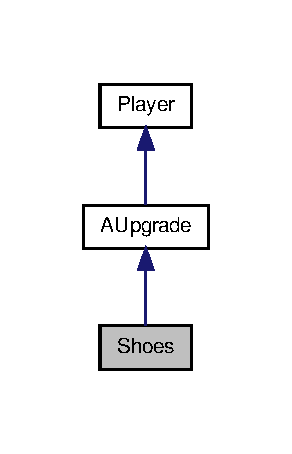
\includegraphics[width=140pt]{class_shoes__inherit__graph}
\end{center}
\end{figure}
\subsection*{Public Member Functions}
\begin{DoxyCompactItemize}
\item 
\hyperlink{class_shoes_a6f99c3ade2822f764a2e658ad5d97dca}{Shoes} (\hyperlink{class_player}{Player} $\ast$character, int pos\-X, int pos\-Y)
\begin{DoxyCompactList}\small\item\em Default constructor. \end{DoxyCompactList}\item 
\hypertarget{class_shoes_afc511aaebac8e7ab57286cf35db7ce8f}{virtual \hyperlink{class_shoes_afc511aaebac8e7ab57286cf35db7ce8f}{$\sim$\-Shoes} ()}\label{class_shoes_afc511aaebac8e7ab57286cf35db7ce8f}

\begin{DoxyCompactList}\small\item\em Default destructor. \end{DoxyCompactList}\item 
virtual int \hyperlink{class_shoes_a61b25a380629e60aa9996dc05a8db0df}{get\-Jump\-Speed} ()
\begin{DoxyCompactList}\small\item\em Get the jumping speed value. \end{DoxyCompactList}\item 
virtual int \hyperlink{class_shoes_a25361fa44b1f513548fe717b6befd53d}{get\-Jump\-Height} ()
\begin{DoxyCompactList}\small\item\em Get the jumping height value. \end{DoxyCompactList}\item 
virtual int \hyperlink{class_shoes_abfa031d2089d4e9397585c7a36d0490d}{get\-Speed} ()
\begin{DoxyCompactList}\small\item\em Get the speed value. \end{DoxyCompactList}\end{DoxyCompactItemize}
\subsection*{Additional Inherited Members}


\subsection{Detailed Description}
\hyperlink{class_shoes}{Shoes} class. 

\begin{DoxyAuthor}{Author}
Adrien Bodineau and Alexandre Gomes 
\end{DoxyAuthor}
\begin{DoxyVersion}{Version}
1.\-0 
\end{DoxyVersion}


\subsection{Constructor \& Destructor Documentation}
\hypertarget{class_shoes_a6f99c3ade2822f764a2e658ad5d97dca}{\index{Shoes@{Shoes}!Shoes@{Shoes}}
\index{Shoes@{Shoes}!Shoes@{Shoes}}
\subsubsection[{Shoes}]{\setlength{\rightskip}{0pt plus 5cm}Shoes\-::\-Shoes (
\begin{DoxyParamCaption}
\item[{{\bf Player} $\ast$}]{character, }
\item[{int}]{pos\-X, }
\item[{int}]{pos\-Y}
\end{DoxyParamCaption}
)}}\label{class_shoes_a6f99c3ade2822f764a2e658ad5d97dca}


Default constructor. 


\begin{DoxyParams}{Parameters}
{\em character} & Decorated character \\
\hline
{\em pos\-X} & Position x \\
\hline
{\em pos\-Y} & Position y \\
\hline
\end{DoxyParams}


\subsection{Member Function Documentation}
\hypertarget{class_shoes_a25361fa44b1f513548fe717b6befd53d}{\index{Shoes@{Shoes}!get\-Jump\-Height@{get\-Jump\-Height}}
\index{get\-Jump\-Height@{get\-Jump\-Height}!Shoes@{Shoes}}
\subsubsection[{get\-Jump\-Height}]{\setlength{\rightskip}{0pt plus 5cm}int Shoes\-::get\-Jump\-Height (
\begin{DoxyParamCaption}
{}
\end{DoxyParamCaption}
)\hspace{0.3cm}{\ttfamily [virtual]}}}\label{class_shoes_a25361fa44b1f513548fe717b6befd53d}


Get the jumping height value. 

\begin{DoxyReturn}{Returns}
Jumping height value 
\end{DoxyReturn}


Reimplemented from \hyperlink{class_player_a4df8845cc35f7ef2d8aefbeffb141aed}{Player}.

\hypertarget{class_shoes_a61b25a380629e60aa9996dc05a8db0df}{\index{Shoes@{Shoes}!get\-Jump\-Speed@{get\-Jump\-Speed}}
\index{get\-Jump\-Speed@{get\-Jump\-Speed}!Shoes@{Shoes}}
\subsubsection[{get\-Jump\-Speed}]{\setlength{\rightskip}{0pt plus 5cm}int Shoes\-::get\-Jump\-Speed (
\begin{DoxyParamCaption}
{}
\end{DoxyParamCaption}
)\hspace{0.3cm}{\ttfamily [virtual]}}}\label{class_shoes_a61b25a380629e60aa9996dc05a8db0df}


Get the jumping speed value. 

\begin{DoxyReturn}{Returns}
Jump speed value 
\end{DoxyReturn}


Reimplemented from \hyperlink{class_player_a95676c9d2da2c6e778aa8558c5e5fa80}{Player}.

\hypertarget{class_shoes_abfa031d2089d4e9397585c7a36d0490d}{\index{Shoes@{Shoes}!get\-Speed@{get\-Speed}}
\index{get\-Speed@{get\-Speed}!Shoes@{Shoes}}
\subsubsection[{get\-Speed}]{\setlength{\rightskip}{0pt plus 5cm}int Shoes\-::get\-Speed (
\begin{DoxyParamCaption}
{}
\end{DoxyParamCaption}
)\hspace{0.3cm}{\ttfamily [virtual]}}}\label{class_shoes_abfa031d2089d4e9397585c7a36d0490d}


Get the speed value. 

\begin{DoxyReturn}{Returns}
Speed value 
\end{DoxyReturn}


Reimplemented from \hyperlink{class_player_a5755be9818f6f911d9494e4948d8c483}{Player}.


\chapter{File Documentation}
\hypertarget{_a_upgrade_8h}{\section{include/\-Decorator/\-A\-Upgrade.h File Reference}
\label{_a_upgrade_8h}\index{include/\-Decorator/\-A\-Upgrade.\-h@{include/\-Decorator/\-A\-Upgrade.\-h}}
}
\subsection*{Classes}
\begin{DoxyCompactItemize}
\item 
class \hyperlink{class_a_upgrade}{A\-Upgrade}
\begin{DoxyCompactList}\small\item\em Abstract class for the upgrades. \end{DoxyCompactList}\end{DoxyCompactItemize}

\hypertarget{_cape_8h}{\section{include/\-Decorator/\-Cape.h File Reference}
\label{_cape_8h}\index{include/\-Decorator/\-Cape.\-h@{include/\-Decorator/\-Cape.\-h}}
}
\subsection*{Classes}
\begin{DoxyCompactItemize}
\item 
class \hyperlink{class_cape}{Cape}
\begin{DoxyCompactList}\small\item\em \hyperlink{class_cape}{Cape} upgrade. \end{DoxyCompactList}\end{DoxyCompactItemize}

\hypertarget{_player_8h}{\section{include/\-Decorator/\-Player.h File Reference}
\label{_player_8h}\index{include/\-Decorator/\-Player.\-h@{include/\-Decorator/\-Player.\-h}}
}
\subsection*{Classes}
\begin{DoxyCompactItemize}
\item 
class \hyperlink{class_player}{Player}
\begin{DoxyCompactList}\small\item\em \hyperlink{class_player}{Player} class. \end{DoxyCompactList}\end{DoxyCompactItemize}

\hypertarget{_shoes_8h}{\section{include/\-Decorator/\-Shoes.h File Reference}
\label{_shoes_8h}\index{include/\-Decorator/\-Shoes.\-h@{include/\-Decorator/\-Shoes.\-h}}
}
\subsection*{Classes}
\begin{DoxyCompactItemize}
\item 
class \hyperlink{class_shoes}{Shoes}
\begin{DoxyCompactList}\small\item\em \hyperlink{class_shoes}{Shoes} class. \end{DoxyCompactList}\end{DoxyCompactItemize}

\hypertarget{_a_factory_8h}{\section{include/\-Factory/\-A\-Factory.h File Reference}
\label{_a_factory_8h}\index{include/\-Factory/\-A\-Factory.\-h@{include/\-Factory/\-A\-Factory.\-h}}
}
\subsection*{Classes}
\begin{DoxyCompactItemize}
\item 
class \hyperlink{class_a_factory}{A\-Factory}
\begin{DoxyCompactList}\small\item\em Provide a factory to create blocks. \end{DoxyCompactList}\end{DoxyCompactItemize}

\hypertarget{_block_ground1_8h}{\section{include/\-Factory/\-Block\-Ground1.h File Reference}
\label{_block_ground1_8h}\index{include/\-Factory/\-Block\-Ground1.\-h@{include/\-Factory/\-Block\-Ground1.\-h}}
}
\subsection*{Classes}
\begin{DoxyCompactItemize}
\item 
class \hyperlink{class_block_ground1}{Block\-Ground1}
\begin{DoxyCompactList}\small\item\em A concrete block that implements \hyperlink{class_i_block}{I\-Block}. \end{DoxyCompactList}\end{DoxyCompactItemize}

\hypertarget{_block_ground2_8h}{\section{include/\-Factory/\-Block\-Ground2.h File Reference}
\label{_block_ground2_8h}\index{include/\-Factory/\-Block\-Ground2.\-h@{include/\-Factory/\-Block\-Ground2.\-h}}
}
\subsection*{Classes}
\begin{DoxyCompactItemize}
\item 
class \hyperlink{class_block_ground2}{Block\-Ground2}
\begin{DoxyCompactList}\small\item\em Another concrete block that implements \hyperlink{class_i_block}{I\-Block}. \end{DoxyCompactList}\end{DoxyCompactItemize}

\hypertarget{_block_ground3_8h}{\section{include/\-Factory/\-Block\-Ground3.h File Reference}
\label{_block_ground3_8h}\index{include/\-Factory/\-Block\-Ground3.\-h@{include/\-Factory/\-Block\-Ground3.\-h}}
}
\subsection*{Classes}
\begin{DoxyCompactItemize}
\item 
class \hyperlink{class_block_ground3}{Block\-Ground3}
\begin{DoxyCompactList}\small\item\em Another concrete block that implements \hyperlink{class_i_block}{I\-Block}. \end{DoxyCompactList}\end{DoxyCompactItemize}

\hypertarget{_concrete_factory_8h}{\section{include/\-Factory/\-Concrete\-Factory.h File Reference}
\label{_concrete_factory_8h}\index{include/\-Factory/\-Concrete\-Factory.\-h@{include/\-Factory/\-Concrete\-Factory.\-h}}
}
\subsection*{Classes}
\begin{DoxyCompactItemize}
\item 
class \hyperlink{class_concrete_factory}{Concrete\-Factory}
\begin{DoxyCompactList}\small\item\em A concrete factory to create blocks. \end{DoxyCompactList}\end{DoxyCompactItemize}

\hypertarget{_i_block_8h}{\section{include/\-Factory/\-I\-Block.h File Reference}
\label{_i_block_8h}\index{include/\-Factory/\-I\-Block.\-h@{include/\-Factory/\-I\-Block.\-h}}
}
\subsection*{Classes}
\begin{DoxyCompactItemize}
\item 
class \hyperlink{class_i_block}{I\-Block}
\begin{DoxyCompactList}\small\item\em Interface that will be implemented by all the different kinds of blocks. \end{DoxyCompactList}\end{DoxyCompactItemize}

\hypertarget{_game_manager_8h}{\section{include/\-Singleton/\-Game\-Manager.h File Reference}
\label{_game_manager_8h}\index{include/\-Singleton/\-Game\-Manager.\-h@{include/\-Singleton/\-Game\-Manager.\-h}}
}
\subsection*{Classes}
\begin{DoxyCompactItemize}
\item 
class \hyperlink{class_game_manager}{Game\-Manager}
\begin{DoxyCompactList}\small\item\em Provide an instance to manage the game. \end{DoxyCompactList}\end{DoxyCompactItemize}

\hypertarget{_menu_8h}{\section{include/\-Singleton/\-Menu.h File Reference}
\label{_menu_8h}\index{include/\-Singleton/\-Menu.\-h@{include/\-Singleton/\-Menu.\-h}}
}
\subsection*{Classes}
\begin{DoxyCompactItemize}
\item 
class \hyperlink{class_menu}{Menu}
\begin{DoxyCompactList}\small\item\em Game menu. \end{DoxyCompactList}\end{DoxyCompactItemize}

\hypertarget{_i_level_8h}{\section{include/\-Strategy/\-I\-Level.h File Reference}
\label{_i_level_8h}\index{include/\-Strategy/\-I\-Level.\-h@{include/\-Strategy/\-I\-Level.\-h}}
}
\subsection*{Classes}
\begin{DoxyCompactItemize}
\item 
class \hyperlink{class_i_level}{I\-Level}
\begin{DoxyCompactList}\small\item\em Interface that will be implemented by the levels. \end{DoxyCompactList}\end{DoxyCompactItemize}

\hypertarget{_level_one_8h}{\section{include/\-Strategy/\-Level\-One.h File Reference}
\label{_level_one_8h}\index{include/\-Strategy/\-Level\-One.\-h@{include/\-Strategy/\-Level\-One.\-h}}
}
\subsection*{Classes}
\begin{DoxyCompactItemize}
\item 
class \hyperlink{class_level_one}{Level\-One}
\begin{DoxyCompactList}\small\item\em Implements the first level of the game. \end{DoxyCompactList}\end{DoxyCompactItemize}

\hypertarget{_level_two_8h}{\section{include/\-Strategy/\-Level\-Two.h File Reference}
\label{_level_two_8h}\index{include/\-Strategy/\-Level\-Two.\-h@{include/\-Strategy/\-Level\-Two.\-h}}
}
\subsection*{Classes}
\begin{DoxyCompactItemize}
\item 
class \hyperlink{class_level_two}{Level\-Two}
\begin{DoxyCompactList}\small\item\em Implements the second level of the game. \end{DoxyCompactList}\end{DoxyCompactItemize}

%--- End generated contents ---

% Index
\newpage
\phantomsection
\addcontentsline{toc}{part}{Index}
\printindex

\end{document}
